% --- Template for thesis / report with tktltiki2 class ---
% 
% last updated 2013/02/15 for tkltiki2 v1.02

\documentclass[english]{tktltiki2}

% tktltiki2 automatically loads babel, so you can simply
% give the language parameter (e.g. finnish, swedish, english, british) as
% a parameter for the class: \documentclass[finnish]{tktltiki2}.
% The information on title and abstract is generated automatically depending on
% the language, see below if you need to change any of these manually.
% 
% Class options:
% - grading                 -- Print labels for grading information on the front page.
% - disablelastpagecounter  -- Disables the automatic generation of page number information
%                              in the abstract. See also \numberofpagesinformation{} command below.
%
% The class also respects the following options of article class:
%   10pt, 11pt, 12pt, final, draft, oneside, twoside,
%   openright, openany, onecolumn, twocolumn, leqno, fleqn
%
% The default font size is 11pt. The paper size used is A4, other sizes are not supported.
%
% rubber: module pdftex

% --- General packages ---

\usepackage[utf8]{inputenc}
\usepackage[T1]{fontenc}
\usepackage{lmodern}
\usepackage{microtype}
\usepackage{amsfonts,amsmath,amssymb,amsthm,booktabs,color,enumitem,graphicx}
\usepackage[pdftex,hidelinks]{hyperref}
\usepackage{fixltx2e}

% Automatically set the PDF metadata fields
\makeatletter
\AtBeginDocument{\hypersetup{pdftitle = {\@title}, pdfauthor = {\@author}}}
\makeatother

% --- Language-related settings ---
%
% these should be modified according to your language

% babelbib for non-english bibliography using bibtex
\usepackage[fixlanguage]{babelbib}

% add bibliography to the table of contents
\usepackage[nottoc]{tocbibind}

% --- Theorem environment definitions ---

\newtheorem{thm}{Theorem}
\newtheorem{lem}[thm]{Lemma}
\newtheorem{cor}[thm]{Corollary}

\theoremstyle{definition}
\newtheorem{definition}[thm]{Definition}

\theoremstyle{remark}
\newtheorem*{remark}{Remark}


% --- tktltiki2 options ---
%
% The following commands define the information used to generate title and
% abstract pages. The following entries should be always specified:

\title{Distributed Association Rule Discovery from Big Data}
\author{Jiri Hamberg}
\date{\today}
\level{Master's Thesis}
\abstract{Abstract.}

% The following can be used to specify keywords and classification of the paper:

\keywords{keyword 1, keyword 2, keyword 3}

% classification according to ACM Computing Classification System (http://www.acm.org/about/class/)
% This is probably mostly relevant for computer scientists
% uncomment the following; contents of \classification will be printed under the abstract with a title
% "ACM Computing Classification System (CCS):"
% \classification{}

% If the automatic page number counting is not working as desired in your case,
% uncomment the following to manually set the number of pages displayed in the abstract page:
%
% \numberofpagesinformation{16 pages + 10 appendix pages}
%
% If you are not a computer scientist, you will want to uncomment the following by hand and specify
% your department, faculty and subject by hand:
%
% \faculty{Faculty of Science}
% \department{Department of Computer Science}
% \subject{Computer Science}
%
% If you are not from the University of Helsinki, then you will most likely want to set these also:
%
% \university{University of Helsinki}
% \universitylong{HELSINGIN YLIOPISTO --- HELSINGFORS UNIVERSITET --- UNIVERSITY OF HELSINKI} % displayed on the top of the abstract page
% \city{Helsinki}
%


\begin{document}

% --- Front matter ---

\frontmatter      % roman page numbering for front matter

\maketitle        % title page
\makeabstract     % abstract page

\tableofcontents  % table of contents

% --- Main matter ---

\mainmatter       % clear page, start arabic page numbering


\section{Introduction}

\textit{Big Data} is a term coined to capture the essence of large datasets typical for the digital age. Big Data can be described by three aspects: \textit{volume}, \textit{velocity} and \textit{variety}, that make such data difficult to process and analyse by traditional tools and methods~\cite{doi:10.1108/LR-06-2015-0061}. Big \textit{volume} means that the data is simply too large to be processed by traditional tools. Big \textit{velocity} means that the data is growing so quickly that traditional tools cannot keep up with the pace. Big \textit{variety} can refer to high dimensionality or loosely constrained structure of a dataset.

Association rule discovery is an established data mining technique that is commonly used to discover interesting relations from a dataset without making assumptions about its structure. This thesis work explores the applicability of association rule discovery on Big Data. As a practical application of the theory, this thesis will demonstrate how the association rule discovery can be applied to discover relations between mobile device system settings and level of energy consumption from the data produced by Carat~\cite{Oliner:2013:CCE:2517351.2517354}, a collaborative energy diagnosis project.

The Carat project has collected data from over 800,000 mobile devices worldwide since its initiation in 2012~\cite{7840871}. The Carat data is collected from mobile device users that have installed the Carat mobile application to their device. An analysis server collects data samples sent by the Carat mobile applications whenever the battery level of the device changes. The data samples consist of a list of system settings, a list of currently running applications and the current battery level. The analysis server uses the collaborative measurements to identify energy consumption anomalies from the users' applications as well as to estimate the energy consumption of individual applications~\cite{Oliner:2013:CCE:2517351.2517354}.

So far the Carat dataset has not been published in its entirety to ensure the privacy of the participants. As discussed in~\cite{7840871}, it would be helpful for mobile application developers to be able to access the energy consumption data of the users of their application. As a part of this thesis work, a prototype of a Carat developer web API is implemented. The API provides a search engine for mobile application developers, allowing them to search for associations between specific system settings and energy consumption level of the mobile device.   

Key research questions that this thesis attempts to answer are:

\begin{enumerate}
	\item How can association rules be generated efficiently and scalably from Big Data? The solution should be fast enough to be used in a real-time query API. 
	
	\item How to select interesting and useful association rules from the set of all generated rules? 
	
	\item How does the discretization algorithm of continuous variables of the Carat data affect the generated association rules? 
\end{enumerate}  

%Various distributed computing technologies have emerged to tackle the difficulties of processing Big Data. Notably, there are two paradigms of distributed computing that have become increasingly popular over the last decade, namely grid based   


\section{Carat Data} \label{carat data}

The Carat data consists of samples containing mobile device system settings and context factors, current battery level, the list of currently running mobile applications and a user specific identification token unique to each Carat application installation. The Carat mobile application periodically collects these samples, typically when the device's battery level changes~\cite{Oliner:2013:CCE:2517351.2517354}. The application sends all collected samples to the server whenever the user opens it or another sample is taken while the application is open.
%Each Carat user periodically sends these samples to the server, typically when the device's battery level changes~\cite{Oliner:2013:CCE:2517351.2517354}. 

Since we are interested in the effects that the mobile device system settings and context factors have on the energy consumption rate of the device, the samples need to be examined as a time series to estimate the energy drain rate over time. This has been done by grouping all samples according to their user identification token. The grouped tokens are then sorted according to the time that the sample was taken. These sorted samples are then paired up so that the first sample and the second sample make up pair number 1, the second and the third sample make up sample pair number 2 and so forth. These sample pairs are used as the basis of this analysis. The energy rate of a sample pair is calculated as the difference of the samples' battery levels divided by the difference of their time stamps. The set of running applications for a sample pair is decided to be the union of both samples' running applications. For all other system settings and context factors, the more recent sample of the pair is used to determine the context factors and system settings of the sample pair.

Since the Carat data comes from a large number of unsupervised clients, there is no guarantee for the integrity of the data. A faulty device or a hostile client may produce erroneous or tampered data. It is therefore essential to apply proper pre-processing to the data in order to minimize the effect that invalid data points have on further analysis. 

Let us give a brief description of each of the system settings and context factors that were used as part of the analysis. Association analysis requires discrete data, as explained in Chapter~\ref{association analysis}. We therefore describe the way each of these variables is discretized. The following presentation of the data is based on a subset of the Carat data consisting of samples that were collected between 26.8.2016 and 3.10.2016 that had Facebook mobile application running. For increased uniformity and simplicity, the data set only contains samples from clients running Android operating system. 

\subsection{Energy Rate}

Energy rate of a mobile device is the velocity at which the mobile devices battery is discharging. The unit of the energy rate is percentage per second. This means that an energy rate of $0.05\frac{\%}{s}$ would drain the whole battery in just $\frac{100}{0.05 / s} = 2000 s \approx 33 minutes$. Any data points where the energy rate was negative, meaning the device's battery was recharging, were filtered out.

%\begin{figure} %[!htbp]
%	\centering
%	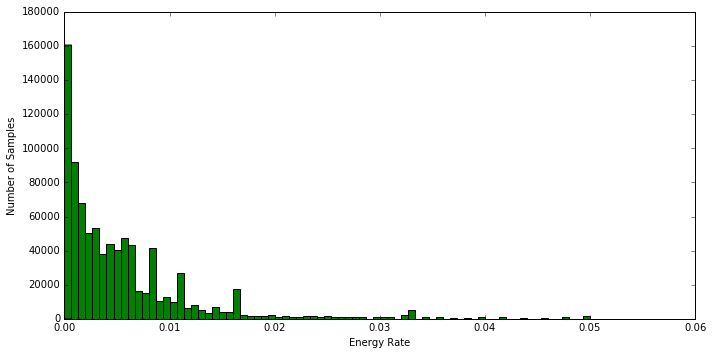
\includegraphics[width=\textwidth]{images/carat-data/energy_rate.png}
%	\caption{Histogram of energy rates with 75 bins}
%	\label{figure:carat-data-energy-rate}
%\end{figure}  
\begin{figure} %[!htbp]
	\centering
	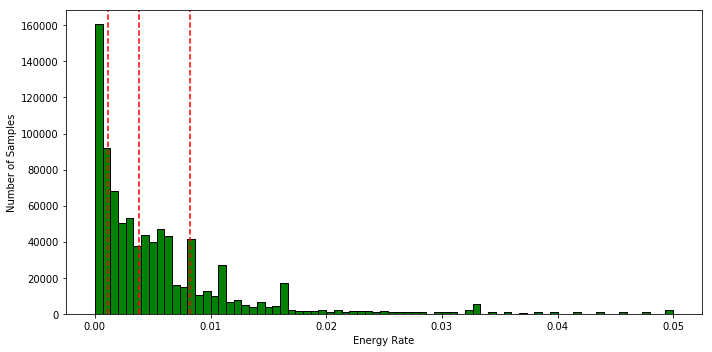
\includegraphics[width=\textwidth]{images/carat-data/energy_rate_w_boundaries.png}
	\caption{Histogram of energy rates with 75 bins in green. The dotted red lines show the boundaries of the four equal mass bins.}
	\label{figure:carat-data-energy-rate}
\end{figure}  


Figure~\ref{figure:carat-data-energy-rate} shows a histogram of the energy rate distribution. The distribution appears to be a rough approximation of an exponential distribution. The distribution does not seem have an evident categorical division. Thus, the data was discretized by dividing it to four bins of equal mass. The discretization boundary points along the energy rate -axis were 0.0011, 0.0038 and 0.0083.

\subsection{CPU Usage Level} \label{carat data cpu} 

CPU usage level is the fraction of time that the central processing unit(s) of the mobile device were busy when the sample was collected. The CPU usage level is in a unit of percentages of the maximum level. All CPU usage levels that were below zero or greater than 1 were discarded as faulty data.

%\begin{figure} %[!htbp]
%	\centering
%	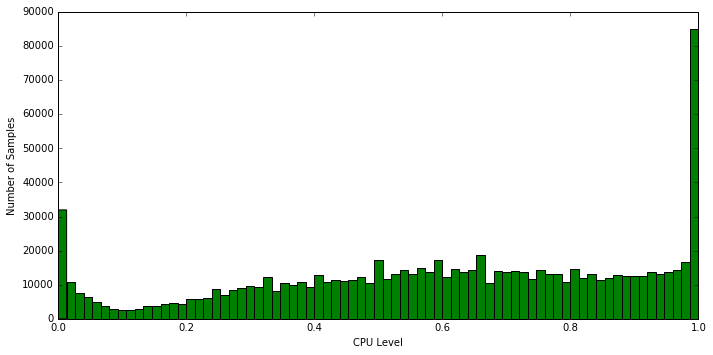
\includegraphics[width=\textwidth]{images/carat-data/cpu_level.png}
%	\caption{Histogram of CPU usage levels with 75 bins}
%	\label{figure:carat-data-cpu-level}
%\end{figure}  
\begin{figure} %[!htbp]
	\centering
	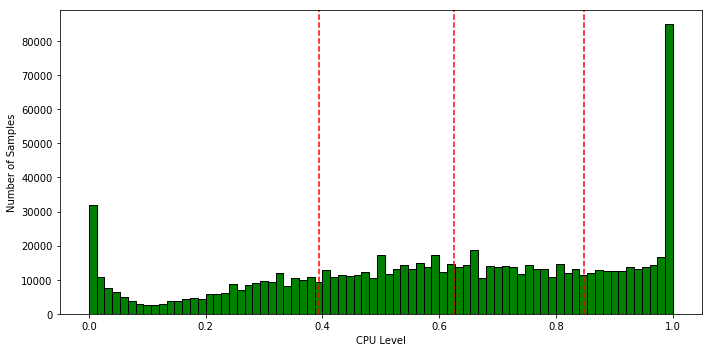
\includegraphics[width=\textwidth]{images/carat-data/cpu_level_w_boundaries.png}
	\caption{Histogram of CPU usage levels with 75 bins in green. The dotted red lines show the boundaries of the four equal mass bins.}
	\label{figure:carat-data-cpu-level}
\end{figure} 

Figure~\ref{figure:carat-data-cpu-level} shows a histogram of the CPU usage level distribution. The distribution very roughly approximates the uniform distribution except for 100\% and 0\% CPU usage levels, which are quite overrepresented. The data was discretized into four bins of equal frequency. The discretization boundary points along the CPU usage -axis were 0.39, 0.63 and 0.85. 

High CPU usage rate has been shown to increase the level mobile device energy consumption~\cite{5375354, PELTONEN201671}, and has been identified as one of the most significant variables in predicting a device's energy consumption. One would therefore assume the CPU utilization level to appear as an antecedent for rules which predict high energy consumption.    

\subsection{Travel Distance}  

Travel distance is the distance in meters, that the mobile device moved between the two samples. Moving mobile phone users have been shown to consume less energy on average compared to stationary ones~\cite{7146507}. This could be due to stationary users being more likely to actively use their devices. 

\begin{figure} %[!htbp]
	\centering
	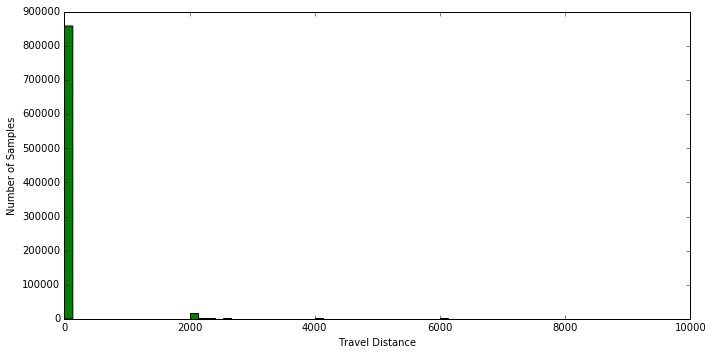
\includegraphics[width=\textwidth]{images/carat-data/travel_distance.png}
	\caption{Histogram of travel distance with 75 bins}
	\label{figure:carat-data-travel-distance}
\end{figure}  

Figure~\ref{figure:carat-data-travel-distance} shows a histogram of the travel distance distribution. Most of the mass of the distribution is concentrated in the close proximity of zero with other values having very low frequencies. The travel distance was discretized to two categories: \textit{moving}, if the travelled distance was greater than 100 meters, and \textit{static} otherwise.

\subsection{Battery Temperature}  

Battery temperature is the measured mobile device battery temperature in degrees Celsius. Temperatures less than five degrees were discarded as it is very rare for a battery temperature to be that low even in subzero climates. Likewise battery temperatures of over 100 degrees were discarded, as healthy devices very rarely reach such high battery temperatures.

%\begin{figure} %[!htbp]
%	\centering
%	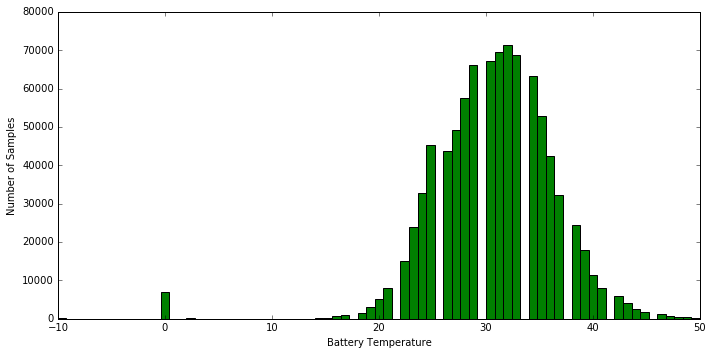
\includegraphics[width=\textwidth]{images/carat-data/battery_temperature.png}
%	\caption{Histogram of battery temperatures with 75 bins}
%	\label{figure:carat-data-battery-temperature}
%\end{figure}  
\begin{figure} %[!htbp]
	\centering
	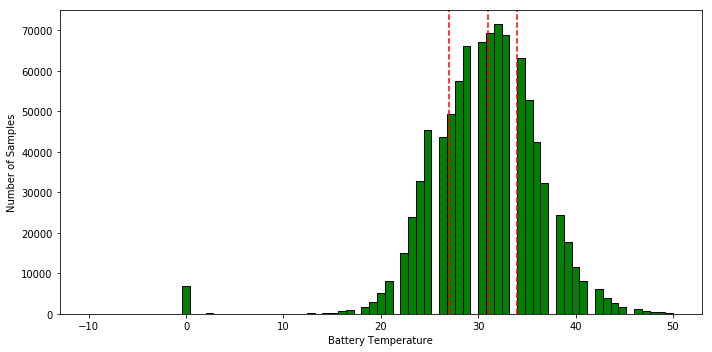
\includegraphics[width=\textwidth]{images/carat-data/battery_temperature_w_boundaries.png}
	\caption{Histogram of battery temperatures with 75 bins in green. The dotted red lines show the boundaries of the four equal mass bins.}
	\label{figure:carat-data-battery-temperature}
\end{figure}

Figure~\ref{figure:carat-data-battery-temperature} shows a histogram of the battery temperature distribution. The distribution approximates a normal distribution with some skewedness. Notably, there is a small cluster of measurements near zero degrees Celsius. This is most likely due to mobile devices systematically reporting a value of zero if the measurement data is not available. The data was discretized into four bins of equal frequency. The discretization boundary points along the battery temperature -axis were 27, 31 and 34. 

High battery temperature has been shown to cause increased battery consumption~\cite{7146507}. The increase in battery temperature cannot always be explained by CPU usage alone, and other factors such as the ambient temperature can affect the battery temperature. It is to be expected that high battery temperature appears as an antecedent of many rules predicting very high energy consumption.
%A straightforward hypothesis would be that a higher battery temperature leads to increased energy rate.

\subsection{Battery Voltage}  

Battery voltage is the electric potential difference generated by the battery in units of volts. Different devices may carry batteries with different voltages. A malfunctioning battery that is near end of its lifetime may give lower than usual voltage readings.

%\begin{figure} %[!htbp]
%	\centering
%	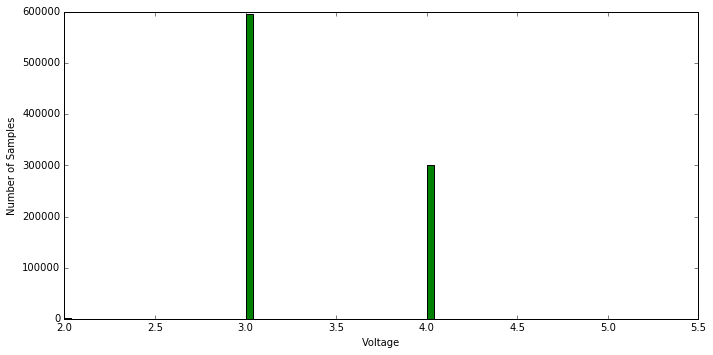
\includegraphics[width=\textwidth]{images/carat-data/battery_voltage.png}
%	\caption{Histogram of battery voltages with 75 bins in green.}
%	\label{figure:carat-data-battery-voltage}
%\end{figure}  
\begin{figure} %[!htbp]
	\centering
	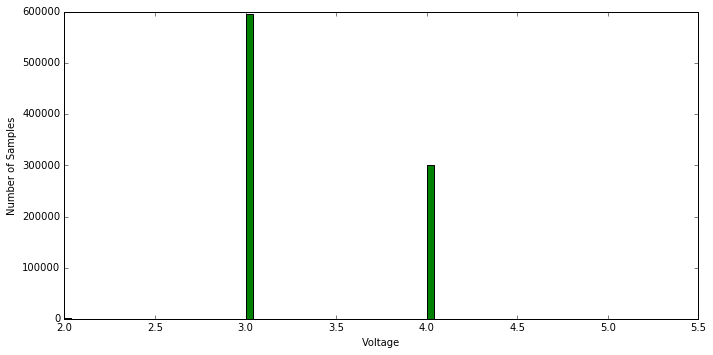
\includegraphics[width=\textwidth]{images/carat-data/battery_voltage.png}
	\caption{Histogram of battery voltages with 75 bins in green.}
	\label{figure:carat-data-battery-voltage}
\end{figure}

Figure~\ref{figure:carat-data-battery-voltage} shows a histogram of battery voltage distribution from the Carat data. The voltages are clustered almost discretely around values of 2, 3 and 4 volts. The voltages were accordingly divided to three bins to reflect this clustering. The discrete voltage data is due to a bug in the Carat data collection software which rounds the readings to integer values. This bug affects the data set used in this thesis work, but has since been fixed. By using a more recent dataset, one would be able to use continuous battery voltage readings in the analysis, which would likely increase the predictive power and accuracy of the generated association rules.         

\subsection{Screen Brightness} \label{carat data screen}

Screen brightness is system setting that takes integer values between -1 and 255. Higher values correspond to higher screen brightness. The value negative one has a special meaning indicating automatic screen brightness, where the screen's brightness is adjusted according to changing illumination of the environment~\cite{PELTONEN201671}.

%\begin{figure} %[!htbp]
%	\centering
%	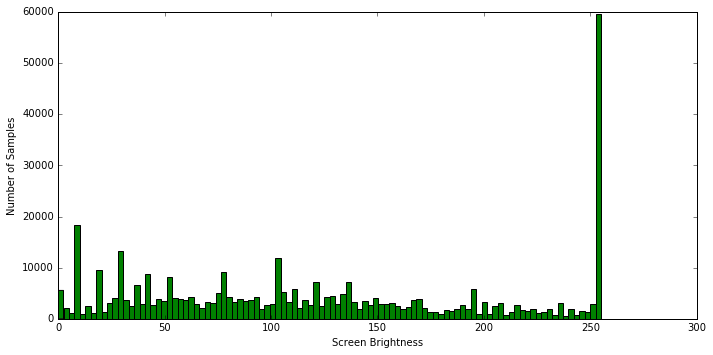
\includegraphics[width=\textwidth]{images/carat-data/screen_brightness.png}
%	\caption{Histogram of screen brightness divided to 100 bins}
%	\label{figure:carat-data-screen-brightness}
%\end{figure}
\begin{figure} %[!htbp]
	\centering
	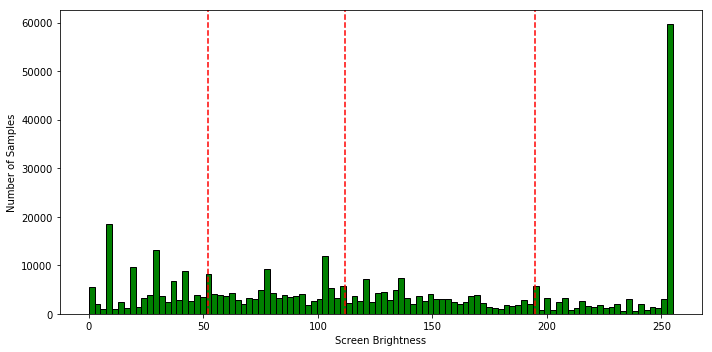
\includegraphics[width=\textwidth]{images/carat-data/screen_brightness_w_boundaries.png}
	\caption{Histogram of screen brightness divided to 100 bins in green. The dotted red lines show to boundary points of the four equal mass bins.}
	\label{figure:carat-data-screen-brightness}
\end{figure}     

Figure~\ref{figure:carat-data-screen-brightness} shows a histogram of the screen brightness values, where the values of -1 have been removed. The brightness values seem to roughly follow a uniform distribution, although very high screen brightness settings seem to be over represented. Approximately half of the samples had their brightness value at -1, indicating automatic brightness setting. Since the automatic setting is categorically different from all other brightness values, the brightness attribute was discretized in the following way: the value -1 formed it's own bin labelled as "auto", while the other numerical values were divided to four bins of equal mass. The boundary points of the equal mass bins along the screen brightness -axis were 52, 112 and 195.   

Increase in screen brightness has been shown to cause increased energy consumption in mobile devices~\cite{5375354, PELTONEN201671} while low and automatically adjusted screen brightness values lead to decrease in energy consumption. It is expected that this phenomena shows up in the association rules as well.

\subsection{Mobile Network Technology}  

The mobile network technology is a system property that reports the name of the mobile technology that mobile device is using for its mobile data communication. Common values include LTE, HSPA, EDGE and UTMS.

\begin{figure} %[!htbp]
	\centering
	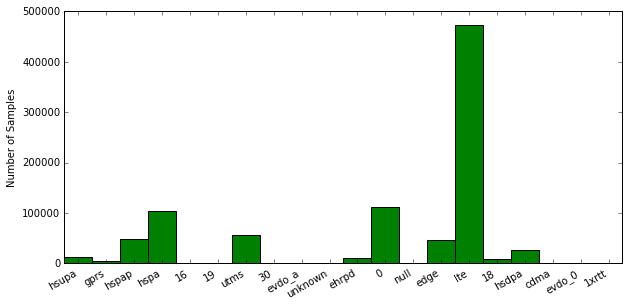
\includegraphics[width=\textwidth]{images/carat-data/mobile_net_type.png}
	\caption{Histogram of mobile network technologies in Carat data.}
	\label{figure:carat-data-mobile-net-type}
\end{figure}   

Figure~\ref{figure:carat-data-mobile-net-type} shows a histogram of all mobile network types in the Carat data. Numeric values were mapped to mobile network type names according to Android developer reference manual~\footnote{https://developer.android.com/reference/android/telephony/TelephonyManager.html}. Ambiguous values such as "unknown", "null" as well as any numerical value not listed in the Android developer reference manual, were combined to a single bin labelled as "unknown". 

Different mobile networking technologies have been shown to have varying energy consumption performance depending on the task~\cite{5357972}. Based on this observation, one would assume that different mobile network technologies should appear as antecedents for association rules predicting either high or low energy consumption depending on the network usage pattern of the mobile application.  

%Intuitively, one would assume that older mobile network technologies such as \textit{gprs} would consume less battery life than newer technologies such as \textit{lte}, since the newer technologies achieve much greater data rates than the old technologies.

\subsection{Network Type}  

Network type is a system property that is reported by the mobile device to indicate the type of the data connection. Typically this is either \textit{mobile} or \textit{wifi}, indicating the use of mobile networking or a wireless local area networking respectively. Some more exotic alternatives can however be found in the data, such as \textit{bluetooth tethering}, where the network access is enabled by bluetooth tunneling through another device.

\begin{figure} %[!htbp]
	\centering
	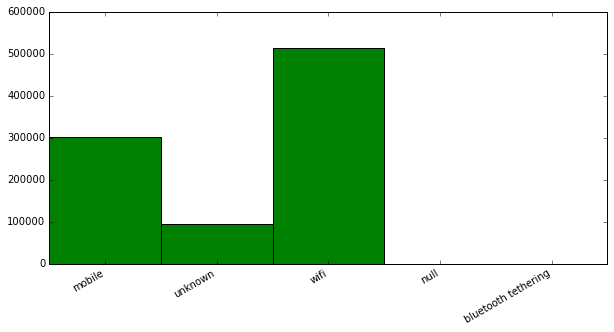
\includegraphics[width=\textwidth]{images/carat-data/network_type.png}
	\caption{Histogram of network types in Carat data}
	\label{figure:carat-data-net-type}
\end{figure}   

Figure~\ref{figure:carat-data-net-type} shows a histogram of all network types found in the Carat data. Values \textit{null} and \textit{unknown} were considered ambiguous and were combined under the label \textit{unknown}.
 
The choice of networking technology has been shown to affect the energy consumption of mobile devices~\cite{7146507, 6240745}. As a general rule, using WiFi network for downloading data is more energy efficient than using a mobile networking technology. Therefore a reasonable hypothesis is to expect to see association rules with mobile networking type as an antecedent for rules predicting high energy consumption, at least in case of applications that download a lot of data.  

\subsection{WiFi Signal Strength}

WiFi signal strength is a system property that the mobile device uses to signify the strength of the wireless local area network. WiFi connection strength is reported as an integer value in the range -100 to 0, where 0 signifies the strongest signal. Presumably, the WiFi signal strength is in units of decibels relative to milliwatt (dBm). The Android API seems to report a value of -127 when no reading is available. Values less than -100 were excluded from the data as these are very unlikely to be real measurements.

% \begin{figure} %[!htbp]
%	\centering
%	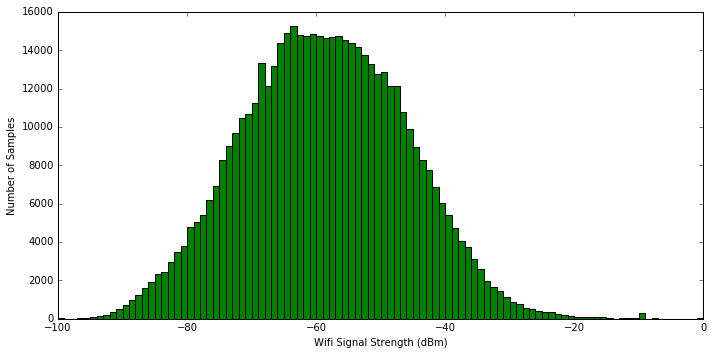
\includegraphics[width=\textwidth]{images/carat-data/wifi_signal_strength.png}
%	\caption{Histogram of WiFi signal strengths readings with 100 bins in Carat data}
%	\label{figure:carat-data-wifi-signal-strength}
%\end{figure}
\begin{figure} %[!htbp]
	\centering
	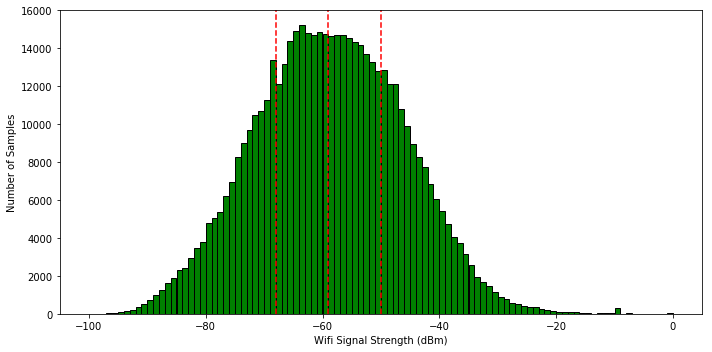
\includegraphics[width=\textwidth]{images/carat-data/wifi_signal_strength_w_boundaries.png}
	\caption{Histogram of WiFi signal strengths readings with 100 bins in green. The dotted red lines show the boundaries of the four equal mass bins.}
	\label{figure:carat-data-wifi-signal-strength}
\end{figure} 

Figure~\ref{figure:carat-data-wifi-signal-strength} shows a histogram of WiFi signal strengths in Carat data. The distribution seems to approximate a normal distribution reasonably well. The data was discretized in four bins with equal mass, the boundaries of which were -68.0, -59.0 and -50.0.

Poor WiFi signal strength has been shown to decrease battery life of mobile devices~\cite{7146507}. This is likely due to increase in the noisiness of the connection, leading to increased data loss and retransmissions, which require extra energy. This effect is expected to be seen in the association rules generated for applications that rely heavily on networking.
%One hypothesis for the interactions between the signal strength and energy rate would be that lower signal strength leads to higher energy rate, as low signal strength s generally increase the noisiness of the connection, leading to increased data loss and retransmissions, which require extra battery life.

\subsection{WiFi Link Speed}

WiFi link speed is a system property that the mobile device uses to report the current wireless local area network link speed. The link speed is presumably reported in units of mega bits per second (mbps). 

WiFi link speed has been shown to have an impact on the mobile device energy consumption~\cite{7146507, 5375354}. Increase in link speed seems to lead to an increase in energy consumption, although this connection does not appear to be nearly as significant as WiFi signal strength for example. The slight increase in energy consumption might be due to users with faster link being able to consume downloadable content more quickly, thus draining the battery more efficiently.
%\begin{figure} %[!htbp]
%	\centering
%	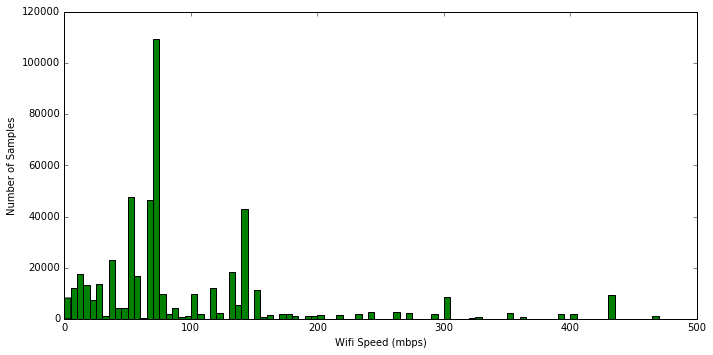
\includegraphics[width=\textwidth]{images/carat-data/wifi_speed.png}
%	\caption{Histogram of WiFi link speed with 100 bins in Carat data}
%	\label{figure:carat-data-wifi-speed}
%\end{figure}

Figure~\ref{figure:carat-data-wifi-speed} shows a histogram of the WiFi link speeds in the Carat data. The link speeds were divided to four bins of equal mass. The boundary points of the bins along the link speed -axis were 54.0, 72.0 and 130.0. 

\begin{figure} %[!htbp]
	\centering
	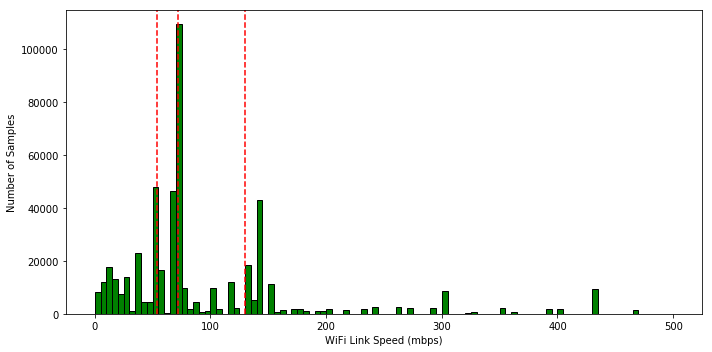
\includegraphics[width=\textwidth]{images/carat-data/wifi_speed_w_boundaries.png}
	\caption{Histogram of WiFi link speed with 100 bins in green. The dotted red lines show the boundary points of the four equal mass bins.}
	\label{figure:carat-data-wifi-speed}
\end{figure}

\section{Association Analysis} \label{association analysis}

Association rule mining is the task of finding associations between \textit{items} in a database of \textit{transactions}. The technique was originally developed in 1993 to identify patterns in consumers grocery purchasing behaviour. Since then however, association analysis has found applications in wide variety of domains.

Let us consider a hypothetical dataset shown in table~\ref{table:raw-data}. The dataset consists of mobile device system settings and energy usage measurements. The dataset has three continuous valued variables:  energyRate, the rate at which the battery is discharging;  CPULevel, the device's CPU usage level and screenBrightness, the brightness of the device's screen. Each of these variables takes floating point values ranging from 0 to 1.
\begin{table}[htb]
    \begin{tabular}{ | l | l | l | }
    \hline
    \textbf{energyRate} & \textbf{CPULevel} & \textbf{screenBrightness} \\ \hline
    0.21 & 0.58 & 0.30 \\ \hline 
    0.80 & 0.46 & 0.61 \\ \hline 
    0.76 & 0.65 & 0.93 \\ \hline 
    0.58 & 0.99 & 0.54 \\ \hline 
    \end{tabular}
	\caption{Hypothetical mobile device measurements inspired by Carat dataset}
	\label{table:raw-data}
\end{table}

Since association rule mining requires each variable of the database to be binary valued, a discretization of the variables must be performed. To discretize a continuously valued variable, we need to replace the continuous variable with multiple binary valued variables, each corresponding to an interval or cluster of values of the continuous variable. The details of discretization are discussed in chapter ???. For now, let us consider a naive discretization strategy, where each continuous variable is split to two binary variables by creating two bins at cut point 0.5. Table~\ref{table:discreteData} demonstrates this idea.

\begin{table}[htb]
    \begin{tabular}{ | l | l | l | l | l | l | }
    \hline
    \textbf{energy=low} & \textbf{energy=high} & \textbf{CPU=low} & \textbf{CPU=high} & \textbf{screen=low} & \textbf{screen=high} \\ \hline
    True & False & False & True & True & False \\ \hline 
    False & True & True & False & False & True \\ \hline 
    False & True & False & True & False & True \\ \hline 
    False & True & False & True & False & True \\ \hline 
    \end{tabular}
	\caption{Hypothetical mobile device measurements after naive discretization}
	\label{table:discreteData}
\end{table}

Since every group of variables that is created by discretization is mutually exclusive, a more concise notation for this dataset can be used, as shown in table~\ref{table:discreteDataConcise}.

\begin{table}[htb]
    \begin{tabular}{ | l | l | l |}
    \hline
	\textbf{energyRate} & \textbf{CPULevel} & \textbf{screenBrightness} \\ \hline
    low & high & low  \\ \hline 
    high & low & high \\ \hline 
    high & high & high \\ \hline 
    high & high & high \\ \hline 
    \end{tabular}
    \caption{Hypothetical mobile device measurements after discretization using concise notation}
    \label{table:discreteDataConcise}
\end{table} 

%As an example, consider a hypothetical database of following transactions denoting individual mobile device system settings, extracted from the Carat data:
 
%\begin{center}
%    \begin{tabular}{ | l | l | }
%    \hline
%    \textbf{Items} \\ \hline
%    cpuLevel=high, energyRate=high \\ \hline 
%    diapers, beer, cookies \\ \hline 
%    diapers, beer, bread \\ \hline 
%    butter, bread, cheese \\ \hline 
%    \end{tabular}
%\end{center} 
 
%The goal of the association analysis is then to produce a list of association rules, given a some measure of interestingness. From the database given above, some algorithm might produce the following association rules: 

Having transformed the raw data to binary variables, the goal of the association analysis is then to produce a list of association rules, given some measure of interestingness. For the database given above, an association rule mining algorithm might find the following association rule 

\[
	\left\{ CPULevel=high, screenBrightness=high \right\} \Rightarrow \left\{ energyRate=high \right\}
\]

This rule implies that high CPU utilization together with high screen brightness associates with high level of battery consumption.

\subsection{Formal Problem Definition}

Let $I = \left\{ x_1, x_2, ..., x_n \right\}$ be a set of binary variables called items. A transaction database $T$ is then a multiset of subsets of $I$, where each element of $T$ denotes a transaction. To give the exact problem of association rule discovery, concepts of support and confidence need to be introduced.

Support of an item set $X$ in database $T$ is defined as the fraction of all transactions in $T$ that contain the item set~\cite{Hipp:2000:AAR:360402.360421}.

\[ supp(X) = \dfrac{ \vert \left\{ X' \in T  \mid X \subseteq X'  \right\}  \vert }{ \vert T \vert  } \]

Confidence of a rule $X \Rightarrow Y$, where $X$ and $Y$ are item sets of $T$, is defined as the fraction of transactions in $T$ containing item set $X$ which also contain $Y$~\cite{Hipp:2000:AAR:360402.360421}.

\[conf( X \Rightarrow Y) = \dfrac{ supp( X \bigcup Y ) }{ supp(X) } \]

The problem of association rule discovery can now be formalized the following way. Given a transaction database $T$, minimum support level $s$, where $ 0 \leq s \leq 1 $ and minimum confidence level $c$, where $ 0 \leq c \leq 1 $, find all rules $X \Rightarrow Y$ where $conf( X \Rightarrow Y ) \geq c$, $supp(X) \geq s$ and $supp(Y) \geq s$~\cite{Hipp:2000:AAR:360402.360421}. 

The association rule discovery problem can be further divided into two distinct sub problems, namely frequent pattern mining problem and rule generation problem. A frequent pattern $P$ of database $T$ is a subset of $I$ such that $supp(P) \geq s$. The frequent pattern mining problem is the task of finding all frequent patterns from a given database. The rule generation problem on the other hand, is the task of generating all association rules with sufficient confidence from the frequent patterns. 

\subsection{Frequent Pattern Mining Using Frequent Pattern Growth}

Frequent pattern growth is an efficient algorithm for the frequent pattern mining problem~\cite{Han:2000:MFP:335191.335372}. The algorithm utilizes a specialized data structure called FP-tree, a kind of prefix tree, to speed up the frequent pattern generation. The FP-tree data structure consists of nodes, each of which have tree fields: item name, item count and node link. The item name tells which item the node represents. The item count signifies the number of transactions containing the item, that can be reached by following the path of nodes in the FP-tree leading to this node. The node link contains a pointer to the next node in the FP-tree with the same node name. An exception to this format is the root node of the FP-tree, which does not have any of these fields, but only has links to child nodes. Algorithm~\ref{Algorithm:FP-tree} shows how to constructs a FP-tree for a transaction database~\cite{Han:2000:MFP:335191.335372}.

\begin{algorithm}[!htbp]
	\SetAlgoLined\DontPrintSemicolon
	\SetKwFunction{buildFPTree}{buildFPTree}\SetKwFunction{insertTree}{insertTree}
	\KwData{A transaction database \textit{DB}, minimum support threshold \textit{s}}
	\KwResult{FP-tree for the database}
	\SetKwProg{myalg}{Algorithm}{}{}
	\myalg{\buildFPTree{}}{
		\nl	\textit{F} $\leftarrow$ Scan \textit{DB} and collect a map of items and their frequencies\;
		\nl \textit{L} $\leftarrow$ Sort keys of \textit{F} in descending order of support filtering out items which have support < \textit{s}\;
		\nl \textit{T} $\leftarrow$ root node of the FP-tree\;
		\nl \For{ transaction \textit{Trans} \textbf{in} \textit{DB} }{ 
			\nl sort \textit{Trans} according to \textit{L} and filter out infrequent items\;
			\nl insertTree(\textit{Trans}, \textit{T})\;
		}
		\nl \KwRet{\textit{T}}\;
	}
	\setcounter{AlgoLine}{0}
	\SetKwProg{myproc}{Procedure}{}{}
  	\myproc{\insertTree{\textit{Trans}, \textit{T}}}{
		\nl \If{\textit{Trans} is empty}{
			\nl \KwRet\;
		} \nl \Else{
			\nl	\textit{N} $\leftarrow$ first item of \textit{Trans}\;
			\nl \textit{tail} $\leftarrow$ tail of \textit{Trans}\;	
			\nl \If{ \textit{T} has a child \textit{h} such that \textit{N}.item-name == \textit{h}.item-name} {
				\nl \textit{h}.count += 1\;
				\nl insertTree(\textit{tail}, \textit{h})
			} \nl \Else {
				\nl \textit{n} $\leftarrow$ create new node with item-name = \textit{p}.item-name and count = 1 and link \textit{T} as its parent\;
				\nl insertTree(\textit{tail}, \textit{n})
			}
		}
	}	
	\caption{Fp-tree construction}
	\label{Algorithm:FP-tree}
\end{algorithm}  

The algorithm consists of two procedures. The entry point for the algorithm is the \textit{buildFPTree}-procedure, which takes no parameters and returns the newly built FP-tree. The sub-program \textit{insertTree} takes a transaction \textit{Trans}, that is sorted by descending item frequency, and an incomplete FP-tree \textit{T} as its parameters. The \textit{insertTree} procedure walks down \textit{T} in a path determined by the items in \textit{Trans}, incrementing the counts of nodes on the path. If there is no existing path to walk down on at any point, the \textit{insertTree} creates a new node with count 1 as a child of the last node that was walked over.

The \textit{buildFPTree} procedure proceeds the following way. In line 1, the transaction database is scanned and the different item names together with their frequencies are collected to variable \textit{F}. In line 2, keys of \textit{F} are sorted in descending order of support and items which have support less than minimum support \textit{s}. The sorted and filtered key-count-pairs are stored in variable \textit{L}. In line 3, the root of node of the FP-tree is created and stored in variable \textit{T}. In line 4, a for loop that iterates over each transaction in the transaction database is entered. The loop yields the transactions in a variable called \textit{Trans}. In line 5, the contents of variable \textit{Trans} are sorted according to the ordering induced by \textit{L} and infrequent items (items which have support that is less than \textit{s}) are filtered out of \textit{Trans}. In line 6, the sub-program \textit{insertTree} is called passing parameters \textit{Trans} and \textit{T}. The for loop entered on line 4 is exited. Finally on line 7, \textit{T}, which now contains the complete FP-tree, is returned.  

The \textit{insertTree} procedure consists of the following steps. In lines 1-3, we check if parameter \textit{Trans} is empty and return if so. In lines 4-5, we store the first item of parameter \textit{Trans} in variable \textit{N} and the rest of the items in variable \textit{tail}. In line 6, we enter an if statement with the conditional "\textit{T} has a child \textit{h} such that \textit{h} has the same item name as \textit{N}". In line 7 we increment the count of \textit{N} by one. In line 8 we call \textit{insertTree} recursively with parameters \textit{tail} and \textit{h}. In line 9, we exit the then-branch of the if statement and enter the else-branch. In line 10, we create a new node with item-name equal to \textit{N}, count equal to 1 and we link \textit{T} as the nodes parent. The newly created node is stored in variable \textit{n}. In line 11 we call \textit{insertTree} recursively with \textit{tail} and \textit{n} as its parameters.

To better illustrate the process of building an FP-tree from a transaction database, let us go through an example that uses a simple made up transaction database. First step of building a FP-tree, is to sort each transaction by decreasing order of frequency of its items in the database. Infrequent items are also filtered out based on the minimum support. Table~\ref{table:fp-growth-example1} shows the example transaction database as well as the frequent items in descending order of frequency. A single traversal over the database is required in order to sort the transactions.

For this example, let us consider a minimum support of 0.3. Since the number of transactions in our database is 6 and $ \frac{1}{6} < 0.3 < \frac{2}{6} $, all items with frequency less than 2 can be filtered out. Thus items i and j are not included in the second column of table~\ref{table:fp-growth-example1}. 

\begin{table}[!htbp]
\begin{center}
    \begin{tabular}{ | l | l | }
    \hline
	\textbf{Items} & \textbf{Frequency Ordered and Filtered Items} \\ \hline
    a, b, c, d, e, h & c, e, h, a, b, d \\ \hline 
    c, d, e, h & c, e, h, d \\ \hline 
    c, e, h & c, e, h \\ \hline 
    a, b, c, e, j & c, e, a, b \\ \hline 
    c, h & c, h \\ \hline
    d, i & d \\ \hline
    \end{tabular}
    \caption{Example transaction database for illustrating FP-tree generation.}
    \label{table:fp-growth-example1}
\end{center}
\end{table} 

To construct the FP-tree we start with a node labelled as "root". We then take the first transaction and walk over its elements in the frequency order. We start from the root node of the FP-tree. Since the roo node has no child nodes, we add a child node labelled with "c" and set its count to 1. We remove the item "c" from the transaction being handled. Then we continue the walk from the node labelled with "c". The procedure is repeated with the remaining items of the transaction, continuing the walk from the node labelled "c". The FP-tree after processing the first transaction is shown in Figure~\ref{figure:fp-growth-example1}.

\begin{figure}[!htbp]
	\centering
	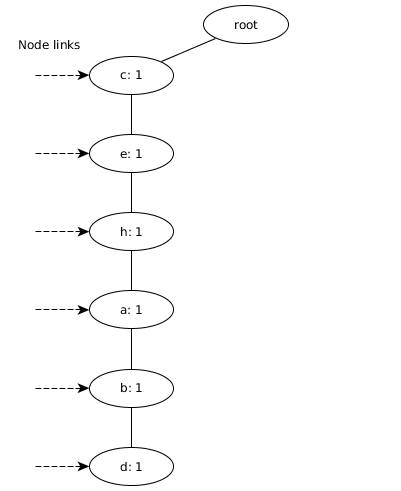
\includegraphics[scale=0.5]{fp-tree-example/fp-tree-p1.png}
	\caption{FP-tree after processing the first transaction}
	\label{figure:fp-growth-example1}
\end{figure}

Next, the second transaction is processed as follows. We again start walking down FP-tree from the root node processing items in the second transaction. Since the root node has a child node labelled with "c" we increment its count to 2 and remove item "c" from the transaction being processed. Since the node has a child node labelled with "e" and our next item to be processed is "e", we move to the node labelled with "e" and increment its count by one and remove item "e" from the transaction being processed. The same process is applied to item "h" and the node labelled with "h". The next item to process is "d", but the node labelled with "h" does not have a child node labelled with "d". We therefore add a child node labelled with "d" and count 1 to the node labelled with "h". Figure~\ref{figure:fp-growth-example2} shows the progress after processing the second transaction of the database.

\begin{figure}[!htbp]
	\centering
	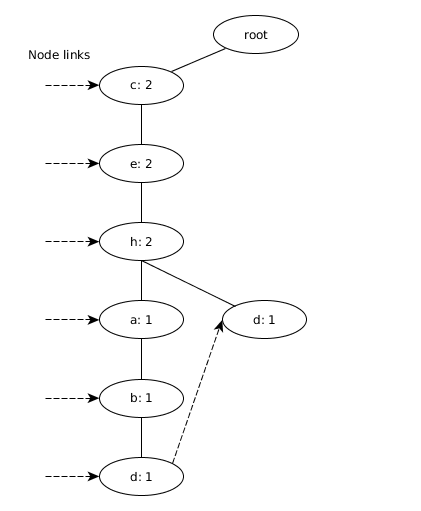
\includegraphics[scale=0.5]{fp-tree-example/fp-tree-p2.png}
	\caption{FP-tree after processing the second transaction}
	\label{figure:fp-growth-example2}
\end{figure}

Repeating the same procedure for the rest of the transactions yields complete FP-tree as illustrated in Figure~\ref{figure:fp-growth-example3}.

\begin{figure}[!htbp]
	\centering
	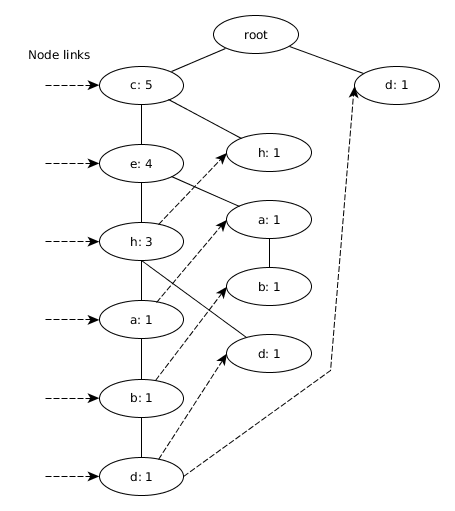
\includegraphics[scale=0.5]{fp-tree-example/fp-tree-p3.png}
	\caption{Complete FP-tree}
	\label{figure:fp-growth-example3}
\end{figure}

The dashed arrows in Figure~\ref{figure:fp-growth-example3} represent node links. The FP-tree maintains a table of linked lists for each distinctly named item. Whenever a node is added to the FP-tree, a pointer to that node is also added to the linked list corresponding to that nodes label.

The way an FP-tree is constructed guarantees, that all FP-trees have the so called \textit{node-link property}~\cite{Hipp:2000:AAR:360402.360421}. What it means, is that for any frequent item, all frequent patterns containing that item can be constructed by following the item's node-links starting from the item's head in the FP-tree header.  

\section{Implementation}

This section discusses the implementation of the Carat developer API prototype. The API aims to provide mobile application developers the ability to discover how a client mobile device's system settings and state affect the energy consumption of the device.

The design of such a service poses multiple challenges, as discussed in~\cite{7840871}. The dataset itself is large and incrementally changing as time passes, which makes static statistical analysis inconvenient. It is therefore practical to design the service in such a way that the analysis can be executed dynamically whenever the API is accessed. Another challenge is to protect the privacy of the participants of the Carat project.

Association rules were selected as the basis of the API for two reasons. First, the association rules effectively hide all the details about individual Carat users, protecting their privacy, while also enabling reasonably detailed view on how a devices system settings and state affect the energy consumption. Secondly, efficient parallel algorithms exist for generating association rules from huge datasets as discussed in detail in chapter~\ref{association analysis}.

As discussed in~\cite{7840871}, the intention of the Carat API is to allow application developers to retrieve information about their application by authenticating with their developer key. The prototype described here, does not include authentication of application developers, but rather demonstrates the functionality that the API could offer provided that an authentication has been successfully completed. 

\begin{figure}[!htbp]
	\centering
	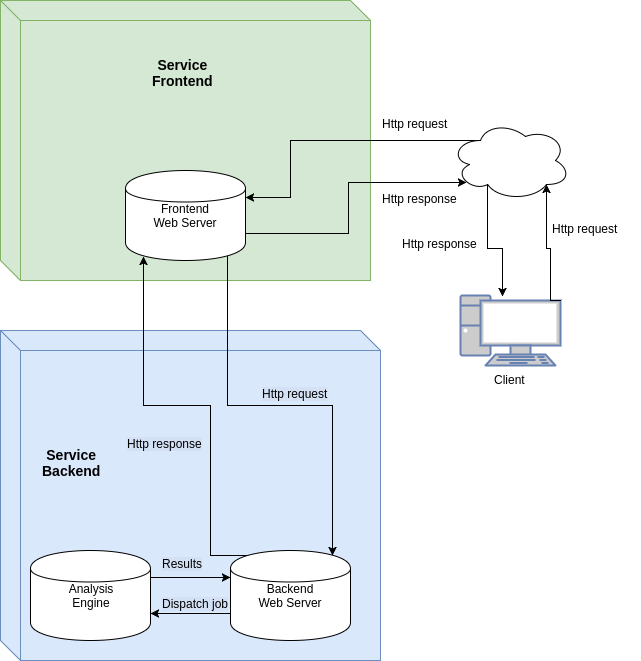
\includegraphics[width=\textwidth]{images/carat-prototype-architecture.png}
	\caption{High level network architecture of the Carat API prototype}
	\label{figure:carat-api-network-prototype}
\end{figure}         

The implementation consists of three main components. These are the front end web server, back end web server and the analysis engine. Figure~\ref{figure:carat-api-network-prototype} shows network level layout of these components and the way these components communicate when the API is accessed. When a client accesses the API, the following flow of requests takes place:
\begin{enumerate}
	\item Client sends a HTTP request to the front end server. The request may contain parameters that control the way the association rules are generated.
	\item Front end web server sends a HTTP request to the back end web server passing along the parameters from the client.
	\item The back end web server dispatches a job to the analysis engine running on SPARK. Parameters provided by the client are used to control the analysis.
	\item Analysis engine sends generated association rules to the back end web server.
	\item Back end server sends HTTP response containing the generated rules to the front end web server.
	\item Front end server uses the association rules to generate a view for the client.  
\end{enumerate}

Figure~\ref{figure:carat-api-network-prototype} shows the flow of control between the different components of the Carat API. The prototype only implements the frontend and the backend of the service. Implementing load balancing and authentication falls outside the scope of this thesis. Some implementation constraints of the authentication module are discussed in~\cite{7840871}.     

\subsection{Service Front End} 

The service front end is implemented using a simple web server written in Scala programming language using Scalatra web framework version 2.4.0 and using Javascript programming language to create the interactive content in the web based graphical user interface. Figure~\ref{figure:frontend-overview} shows to graphical user interface of the service. Initially, a search form will be displayed to the user, containing three input fields for specifying the name of the application to be analysed, the minimum support threshold and the minimum confidence threshold. Additionally, the form contains a check box for each variable to be excluded from the association rule generation. 

\begin{figure}[!htbp]
	\centering
	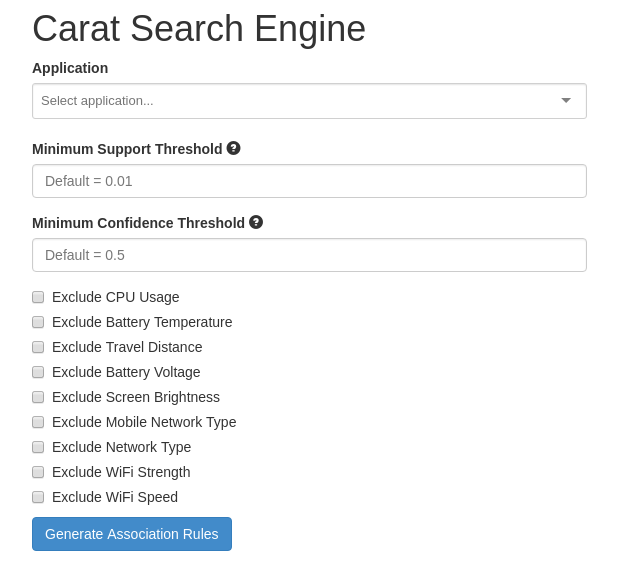
\includegraphics[width=\textwidth]{images/frontend/frontend_overview.png}
	\caption{Overview of the graphical user interface of the front end}
	\label{figure:frontend-overview}
\end{figure} 

The first input field accepts the name of the application. The input field was constructed using selectize.js, a Javascript library for creating searchable drop down lists. As the user starts typing the name of the application in the input field a list of matching application names will be displayed under the input field. By clicking an application name in the list, the user can select the application of interest. To enable this functionality, the application will fetch a list of all available application  when the web page loads using an AJAX request to the web server. Figure~\ref{figure:frontend-selectize} shows how the searching and selecting of applications by name works in practise. In this imaginary scenario, the user is searching applications whose name includes the string "spot". The user is then given a list of options from which to choose. Application names such as "com.spotify.music", "fr.pb.blogspot.com" and "ekawas.blogspot" will be displayed as each of them contain the substring "spot". The matching sections of the names are highlighted in light blue color.    

\begin{figure}[!htbp]
	\centering
	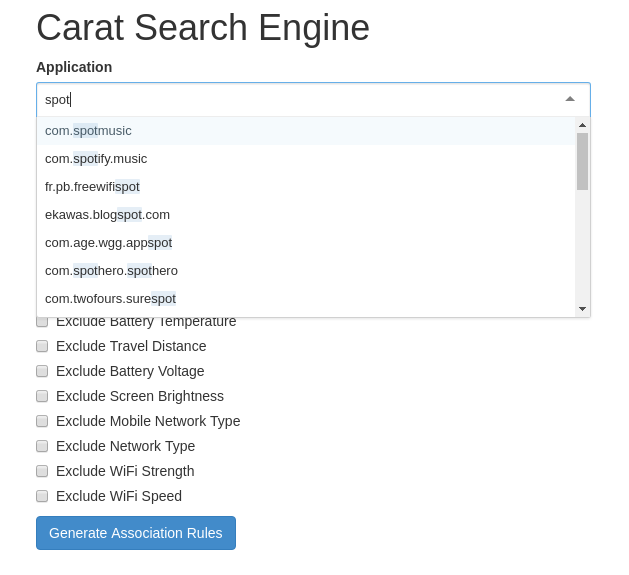
\includegraphics[width=\textwidth]{images/frontend/frontend_selectize.png}
	\caption{Searching and selecting applications by name}
	\label{figure:frontend-selectize}
\end{figure} 

The second and third input fields allow the user to specify the minimum support threshold and the minimum confidence threshold respectively, for the association rule generation. Above above each of these two input fields are icons with question marks. These icons, when hovered over, will display an explanation about the variable in question. This functionality is illustrated in Figure~\ref{figure:frontend-icon-pop-over} for the minimum support threshold. The icon for minimum confidence threshold functions similarly. 

Finally, the form contains a check box for each variable that is included in the association analysis. By checking any of these check boxes, the user can exclude a variable from the analysis. 

\begin{figure}[!htbp]
	\centering
	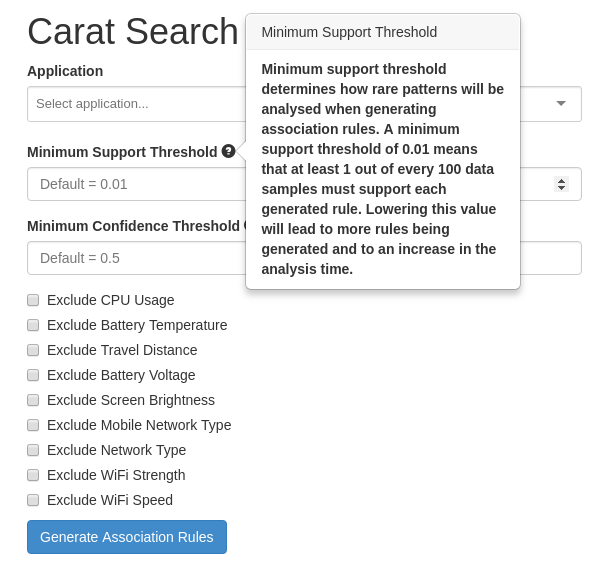
\includegraphics[width=\textwidth]{images/frontend/frontend_helper_icons.png}
	\caption{Helper icon pop over explaining the meaning of minimum support threshold}
	\label{figure:frontend-icon-pop-over}
\end{figure}

Once the user initiates the analysis by pressing the submit button, labelled with "Generate Association Rules", a spinner element is displayed to tell the user that analysis is in process. Once the analysis is complete and the back end returns the analysis results, the spinner element will be removed and the generated rules will be displayed underneath the search form. The rule list is organized in tabs, one for each percentile of the energy rate variable. By clicking on a tab, the rules in which the corresponding energy rate is a consequent, will be displayed. The way the rules are rendered is a simple HTML table, where rules are presented in rows. The first column of the table lists the antecedents of a rule, the second column displays the consequent of a rule and the third column displays the confidence score of a rule. Figure~\ref{figure:frontend-example-rule-list} shows an example of generated rules for the com.facebook.katana mobile application using a minimum support threshold of 0.0001 and a minimum confidence threshold of 0.75. The displayed rules are sorted in an ascending order of confidence to display the most significant rules first.      

\begin{figure}[!htbp]
	\centering
	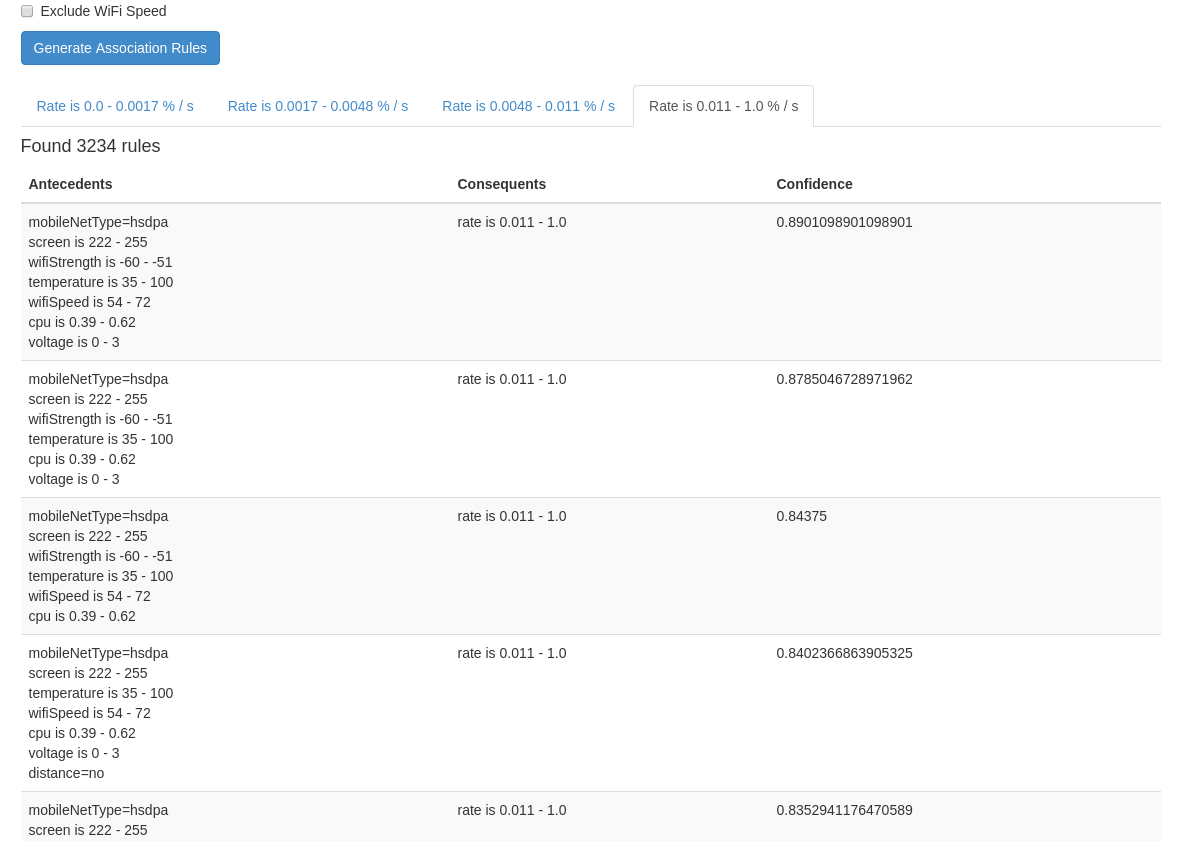
\includegraphics[width=\textwidth]{images/frontend/frontend_rule_list.png}
	\caption{Example of generated  association rules for the com.facebook.katana mobile application. A minimum support threshold of 0.0001 and a confidence threshold of 0.75 was used.}
	\label{figure:frontend-example-rule-list}
\end{figure}

\subsection{Service Back End}

The service back end is a simple web server implemented in Scala programming language using Scalatra web framework version 2.4.0. The webserver listens for HTTP GET requests, accepting application name, minimum support, minimum confidence and a list variable names to be excluded in the requests URL parameters. Once a valid GET request is received, the server creates a Spark job script based on the request parameters, and submits the Spark job to the analysis engine. The shell script which submits the Spark job is executed in a thread pool asynchronously to avoid making the web server unresponsive while a Spark job is running. Once the analysis engine has successfully executed the job, the shell script prints the association rules in JSON format to its standard output stream. This output is captured and returned as a HTTP response to the client.

The server consists of merely three components, a servlet, a service and a bootstrap component. The bootstrap components purpose in Scalatra is to mount services to certain URL paths. The bootstrap component simply mounts our servlet to match with any path, as denoted by asterisk character 
\begin{minipage}{\linewidth}
\begin{lstlisting}[language=scala]
class ScalatraBootstrap extends LifeCycle {
  override def init(context: ServletContext) {
    context.mount(new MainServlet, "/*")
  }
}
\end{lstlisting}
\end{minipage}   

A servlet is a server component that routes incoming requests to associated controller routines. The servlet in question is implemented is Scalatra as follows

\begin{minipage}{\linewidth}
\begin{lstlisting}[language=scala]
class MainServlet extends ScalatraServlet with FutureSupport with JacksonJsonSupport {

  val conf = ConfigFactory.load()
  override val asyncTimeout = conf.getInt("timeout") seconds
  protected implicit lazy val jsonFormats: Formats = DefaultFormats
  implicit val executor = ExecutionContext.global
  
  before() {
    contentType = formats("json")
  }
	
  get("/") {
    val applicationName = Try(params("applicationName")).toOption
	val minSupport = Try(params("minSupport").toDouble).toOption
	val minConfidence = Try(params("minConfidence").toDouble).toOption
    val excluded = Try(params("excluded")).toOption.getOrElse("")

    applicationName.map { applicationName =>
      SparkRunner.runSpark(
        applicationName,
        minSupport = minSupport,
        minConfidence = minConfidence,
        excluded = excluded
      )
    }.getOrElse {
      BadRequest(reason = "Missing 'applicationName'")
    }
  }
}
\end{lstlisting}
\end{minipage}  

The traits \textit{FutureSupport} and \textit{JacksonJsonSupport} indicate, that the response is computed asynchronously and is JSON formatted. The method call to \textit{get("/")} registers a controller routine to the root path of the servlet. The controller routine, which is given as a call-by-name function to the second parameter list of the \textit{get} call, parses URL parameters from the incoming HTTP request and submits a new task to the \textit{SparkRunner} service. In case the \textit{applicationName} is missing from the request, a \textit{BadRequest} HTTP response is produced, otherwise the service method \textit{runSpark} is executed asynchronously and a response will be sent once the analysis engine has accomplished its analysis. For example, suppose that the server is running on localhost and listening on port 8888. Upon receiving a GET request to an URI such as \textit{localhost:8888?applicationName=com.facebook.katana\&minConfidence=0.9}, the servlet would route the request to the controller routine configured under \textit{get("/")}. The routine would parse the URI parameters \textit{applicationName} and \textit{minConfidence} and dispatch a Spark job to the analysis engine by invoking \textit{SparkRunner.runSpark}.  



\subsection{Analysis Engine}

\begin{wrapfigure}{r}{0.35\textwidth}
	\vspace{-110pt}
	\begin{center}
		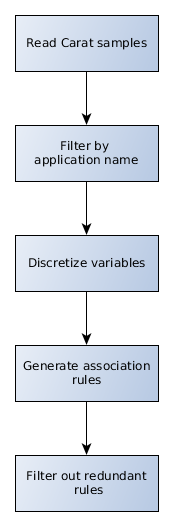
\includegraphics[width=0.3\textwidth]{images/analysis_engine_flow_graph.png}
	\end{center}
	\caption{Overview of the analysis engine pipeline}
	\label{figure:analysis-engine-flow-graph}
\end{wrapfigure}

The primary function of the analysis engine is to generate association rules from the Carat data based on provided query parameters. The query parameters consist of application name, minimum confidence, minimum support and an optional list of attribute names which are to be excluded from the analysis. The application name is used to filter out all Carat energy rate samples in which the the application is not present. The minimum support and minimum confidence parameters affect the association rule generation as described in chapter~\ref{association analysis}. The excluded attributes list controls the association rule generation by completely ignoring all included attributes.    

%\begin{figure}[!htbp]
%	\centering
%	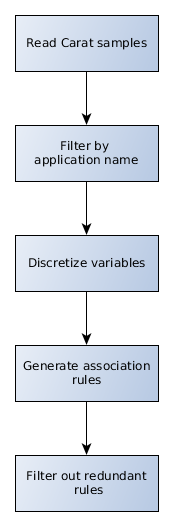
\includegraphics[width=0.25\textwidth]{images/analysis_engine_flow_graph.png}
%	\caption{Overview of the analysis engine pipeline}
%	\label{figure:analysis-engine-flow-graph}
%\end{figure}    
 
Figure~\ref{figure:analysis-engine-flow-graph} describes the process of generating association rules as a simple pipeline consisting of four steps. We will now go through each step providing snippets of code, taken from the analysis engine implementation, that will shed light on the implementation in Spark programming framework. 

Reading Carat samples is very simple in Spark, as is evident from the following code snippet.  

\begin{minipage}{\linewidth}
\begin{lstlisting}[language=scala]
def readCaratRates(sampleDir: String)(implicit sc: SparkContext): RDD[fi.helsinki.cs.nodes.carat.sample.Rate] = {
	sc.objectFile[fi.helsinki.cs.nodes.carat.sample.Rate](s"${sampleDir}")
}
\end{lstlisting}
\end{minipage}

The $objectFile$ method of the $SparkContext$ object will read the dataset from a given directory. The dataset is stored as an RDD (Resilient Distributed Dataset), that is serialized to the disk in a folder given by the $sampleDir$ parameter. RDD is is the data structure that Spark framework uses to store, access and transform distributed datasets. The Carat samples are initially read as instances of class $fi.helsinki.cs.nodes.carat.sample.Rate$. Each $Rate$ object contains two consecutive samples from a mobile device. From these samples, the system settings and running mobile applications can be extracted as described in chapter~\ref{carat data}  

The next task that the analysis engine carry out, is to filter out all Carat rate samples where the requested application was not running. Using the $readCaratRates$ method, one can compose an expression which reads Carat rate data objects, filters out all rate objects that do not have the requested application running and transforms the resulting rate objects to a simplified object type of class $Sample$. 

\begin{minipage}{\linewidth}
\begin{lstlisting}[language=scala]
val samples = readCaratRates(ratePath).collect {
	case rate if rate.allApps().contains(applicationName) => 
		Sample.fromCaratRate(rate)
}
\end{lstlisting}
\end{minipage}  
The $collect$ is a method defined for all instances of class $RDD[T]$ (where $T$ is a type parameter). It is analogous to the $collect$ method from Scala standard library, taking a partial function of signature $PartialFunction[T, U]$  (where $T$ and $U$ are type parameters) and returning a new instance of $RDD[U]$, containing the image of the $RDD[T]$ mapped by the partial function.
        
The $Sample$ is a simple case class that merely stores all the relevant system settings. The case class also has a companion object, in which the method $fromCaratRate$ is defined. The method simply constructs a $Sample$ instance from a $Rate$ instance. 

\begin{minipage}{\linewidth}
\begin{lstlisting}[language=scala]
case class Sample(
	rate: Double,
	cpu: Double,
	distance: Double,
	temp: Double,
	voltage: Double,
	screen: Double,
	mobileNetwork: String,
	network: String,
	wifiStrength: Double,
	wifiSpeed: Double
)
\end{lstlisting}
\end{minipage}  

The next step in the analysis work flow, is to discretize the variables of the data. All numerical variables were discretized to bins of equal mass, as explained in depth in chapter~\ref{carat data}. The following code snippet shows how to find the break points of the bins for continuously valued variables.

\begin{minipage}{\linewidth}
\begin{lstlisting}[language=scala] 
def getQuantiles(
  data: RDD[Double],
  buckets: Int,
  relativeError: Double = 0.0001,
  partial: 
  	PartialFunction[Double, Option[String]] = Map.empty)
  (implicit sqlContext: SQLContext): 
Array[Double] = {
	
  import sqlContext.implicits._

  val percentiles = (for(i <- 1 to (buckets - 1)) yield (1.0 / buckets) * i).toArray
  val notDefined = data.filter(x => !partial.isDefinedAt(x))

  try {
    notDefined.toDF("col").stat.approxQuantile("col", percentiles, relativeError)
  } catch{
    case ex: java.util.NoSuchElementException => Array[Double]()
  }
}
\end{lstlisting}
\end{minipage}  

The method $getQuantiles$ takes as an its input $data$, an $RDD$ containing the values to be discretized; $buckets$, the number of bins to create; $relativeError$, the maximum relative error that is allowed when approximating the break points of the percentiles; $partial$, a partial function that is used to filter out values that should not be taken into account when approximating the percentiles. The method uses Spark $DataFrame$ API to approximate the percentiles. Using a $relativeError$ parameter larger than 0, makes the generation of the association rules non deterministic, since the approximated percentile break points are allowed to vary from the exact value. However, calculating exact values for the breakpoints (by setting the $relativeError$ parameter to zero) slows down the generation of the association rules considerably, as all of the data needs to be processed in order to calculate the break points as opposed to calculating the break points from a sampled dataset.

Having computed the quantiles of a continuously valued variable, discretization can be achieved by using the following method

\begin{minipage}{\linewidth}
\begin{lstlisting}[language=scala] 
def getFeatureFromQuantiles(
	dataPoint: Double,
	featureName: String,
	quantiles: Array[Double],
	partial: PartialFunction[Double, Option[String]] = Map.empty
): Option[String] = {
	if(partial.isDefinedAt(dataPoint))
		return partial(dataPoint).map { x => 
			s"${featureName}=${x}"
		}
	
	var index = quantiles.indexWhere(q => q >= dataPoint) + 1	
	if (index == 0) index += (quantiles.length + 1)
	Some(s"${featureName}=q${index}")
}  
\end{lstlisting}
\end{minipage}  

The method \textit{getFeaturesFromQuantiles} takes as its input \textit{dataPoint}, a single point of data to be discretized; \textit{featureName}, the name of the feature; \textit{quantiles}, the quantile break points for the variable and \textit{partial} a partial function that is used both to filter out invalid data as well as to bypass the discretization altogether.

As a concrete example, let us examine how one could go about discretizing variable \textit{screen}, which gives the screen brightness of the mobile device. As discussed in chapter~\ref{carat data screen}, the variable takes values between -1 and 255, where value -1 signifies a special case, where the screen brightness is automatically adapted to the brightness of the surroundings of the device. One could encode these preconditions to a partial function of the following form:
\begin{minipage}{\linewidth}
\begin{lstlisting}[language=scala] 
val screenPartial: PartialFunction[Double, Option[String]] = {
    case x if x == -1 => Some("auto")
    case x if x < -1 => None
	case x if x > 255 => None
}
\end{lstlisting}
\end{minipage} 
Using this partial function in conjunction with the methods \textit{getQuantiles} and \textit{getFeatureFromQuantiles} for each data point will give the discretized form of the variable \textit{screen}. 

To summarise: in order to discretize a variable such as \textit{screen}, which is assumed to be a collection of type \textit{RDD[Double]}, one could fist calculate the quantiles of data using the method \textit{getFeatureFromQuantiles}. One must then define a partial function, such as the one mentioned above, that filters out invalid data points and handles values with special significance. Finally, the method \textit{getFeatureFromQuantiles} could be applied to each data point of the collection using the partial function and the quantiles.

Having ediscretized all the variables of the dataset, using the procedure discussed above, one ends up with one array of strings for each sample, which is represented in Spark by type \textit{RDD[Array[String]]}. To generate the association rules from these discrete features, MLlib, a machine learning library for Spark was used. The library implements a parallel FPGrowth algorithm for this purpose. The FPGrowth implementation has a limitation however, in that it can only generate rules with single consequent. The limitation is not terribly severe for the purpose of this thesis, as the main interest lies in finding out which variables affect the battery usage. Therefore being limited to rules which have as their sole consequent a feature extracted from the energy rate variable, should be sufficient. The following snippet of code illustrates how to generate association rules using the MLlib API.

\begin{minipage}{\linewidth}
\begin{lstlisting}[language=scala] 
val fpg = new FPGrowth()
		  .setMinSupport(minSupport)
			  
val model = fpg.run(features)

val rulesFiltered = model.generateAssociationRules(minConfidence)
  .filter { rule =>
    rule.consequent.find { item =>
	  item.startsWith("rate=")
	}.isDefined
  }
\end{lstlisting}
\end{minipage}       

The final stage of association rule generation workflow is filtering out redundant rules. To demonstrate what is meant by redundancy in this context, let us consider two rules such as    

\begin{equation}
	\left\{ A, B \right\}  \Rightarrow  \left\{ X \right\} \label{rule:1}
\end{equation}

\begin{equation}
\left\{ A, B, C \right\}  \Rightarrow  \left\{ X \right\} \label{rule:2}
\end{equation}

Additionally, let us assume that both rules \eqref{rule:1} and \eqref{rule:2} have equivalent confidence. Since both rules predict the same consequents and the antecedents of rule \eqref{rule:1} is a subset of the antecedents of rule \eqref{rule:2}, one can conclude that the rule \eqref{rule:1} is the more general of the two rules, as adding item \textit{C} to the antecedents of rule \eqref{rule:1} does not improve the associative power of the original rule. Since the objective of this thesis is to identify variables which have the strongest association with the battery consumption of a mobile application, we consider rule \eqref{rule:2} redundant in the context of this thesis work.

More generally, given a set \textit{S} of association rules, we consider rule $R \in S$ redundant if there exists a rule $r \in S$, such that $R \neq r$ and $r.antedecents \subset R.antedecents$. The following excerpt of code shows how this definition translates to a redundancy filtering algorithm in Scala programming language
    
\begin{minipage}{\linewidth}
\begin{lstlisting}[language=scala] 
def pruneRules(rules: RDD[Rule[String]]): RDD[Rule[String]] = {
  val pruneCandidateGroups = rules.groupBy{ rule => 
    (rule.consequent.sorted.mkString, rule.confidence) 
  }

  pruneCandidateGroups.flatMap { case (key, group) =>
    val groupSorted = group.toSeq.sortBy(rule => rule.consequent.length)
    var groupAsSets = group.map(rule => (rule, rule.antecedent.toSet))

    val toPrune: Set[Rule[String]] = (for {
      testRule <- groupAsSets
      otherRule <- groupAsSets
      if testRule != otherRule && testRule._2.subsetOf(otherRule._2)
    } yield(otherRule._1)).toSet
    
    groupSorted.filter(rule => !toPrune.contains(rule))
  }
}
\end{lstlisting}
\end{minipage}       

Method \textit{pruneRules} takes a collection of association rules and returns a collection of association rules which contains no redundant rules.

This concludes the analysis engine part of the implementation. From usability perspective, generating the association rules should be fast enough not to hinder interactive use, which implies that the rule generation should not take more than a couple of seconds. However, heavily optimizing the analysis engine falls outside the scope of this thesis. In practice, the implementation described here achieves run times of a couple of minutes with a rather modest dataset size of 16 gigabytes.


   

\section{Results}

%The purpose of this thesis work was to design and implement an interactive and semi automated web based tool for discovering association rules from the Carat data that indicate what system settings and usage patterns of a mobile application lead to increased battery consumption. In practise, this has proven to be quite challenging for a number of reasons:

%\begin{itemize}
%  \item Automatically deciding a sufficient threshold for support and confidence for generating rules is difficult 
%  \item Number of generated rules increases rapidly as support and confidence thresholds are lowered
%  \item Identifying interesting or relevant rules in presence of hundreds or thousands of rules is cumbersome
%  \item Deciding how to discretize ordinal and continuous variables is non-trivial          
%\end{itemize}

We will now look at the results of this work in two parts. In the first part we will be looking at the performance of the application and how it affects its usability. In the second part we will take a closer look at some examples of generated rules. The last part of this chapter focuses on the impact of these results and suggests ways to improve on this work. 


\subsection{Performance Evaluation}

\begin{figure} %[htp]

\subfloat[Number of rules with fitted plane]{
  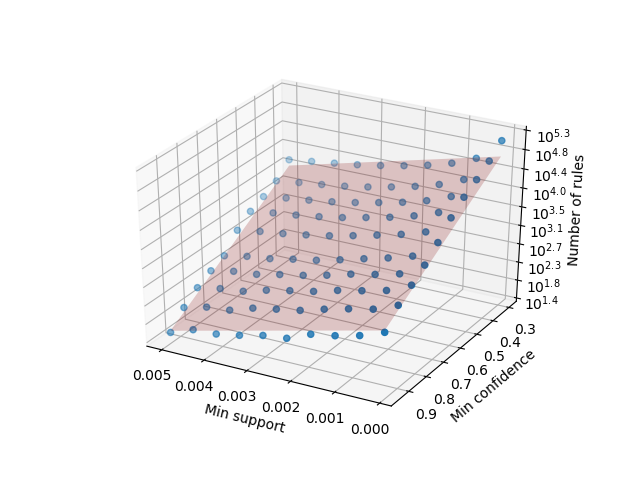
\includegraphics[width=0.95\textwidth]{images/results/facebook_num_rules.png}%
}

\subfloat[Number of rules with error bars]{%
  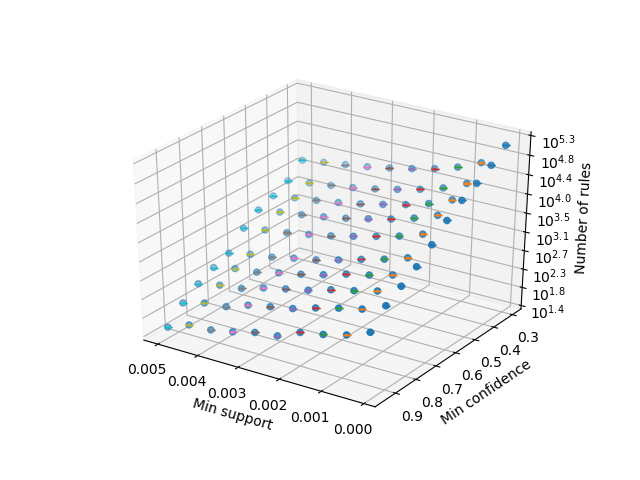
\includegraphics[width=0.95\textwidth]{images/results/facebook_num_rules_with_error_bars.png}%
}

\caption{Number of generated rules for Facebook measurements as a function of minimum support threshold and minimum confidence threshold}
\label{figure:number-of-rules-facebook}
\end{figure}

In order to understand the relationship between the number of generated rules and minimum support and confidence thresholds, a series of measurements were conducted on the Carat API prototype server. Figure~\ref{figure:number-of-rules-facebook} shows these  measurements for Facebook application and Figure~\ref{figure:number-of-rules-spotify} shows the measurements for Spotify application. The figures show the relationship of generated rules as a function of minimum support threshold and confidence threshold as a three dimensional plot. A series of five measurements were conducted for each application. In each of series, a minimum confidence threshold range of 0.3 to 0.9 and a minimum support threshold range of 0.0001 to 0.005 were both divided evenly by 10 points creating a grid of 100 points where the measurements were taken. The blue dots represent average of the five measurement at each point of the support-confidence-grid. In sub figure A, a plane was fitted to the measurements points using least squares method. This was done to better illustrate the spatial configuration of the measurements as well as to showcase how well the measured points are aligned on the plane. In sub figure B, error bars were plotted to the measurements using one standard deviation of the five measurements as the size of the error. 

%Figure~\ref{figure:number-of-ruless} shows the relationship of these variables on two selected applications, namely Spotify and Facebook mobile applications. The blue dots represent individual measurements. A minimum confidence threshold range of 0.3 to 0.9 and a minimum support threshold range of 0.0001 to 0.005 were both divided evenly by 10 points creating a grid of 100 points where the measurements were taken. The number of rules -axis is in $log_{10}$ scale to better illustrate the varying magnitudes of the number of generated rules. The transparent red plane was fitted to the measured points using the least squares method.

The number generated rules seems to grow exponentially on both axes when approaching zero, as can be seen by how well the measurements align with the least squares plane. This explosion in the number of generated rules makes it difficult for the user to extract useful rules from the system when small values for the thresholds are used. To mitigate this problem, the system provides two features:

\begin{itemize}
	\item The generated rules are sorted in the ascending order of their confidence, giving the more reliable rules a greater priority.    
         
	\item Attributes can be excluded from the analysis - potentially greatly reducing the number of generated rules. 
\end{itemize}        

Even though there is a stochastic component in the rule generation, which arises from the sampling of data in the variable discretization stage of the analysis, the number of generated rules does not seem to vary much, as can be seen from the error bars, which are barely visible.  


\begin{figure}[htp]
\subfloat[Number of rules with fitted plane]{
  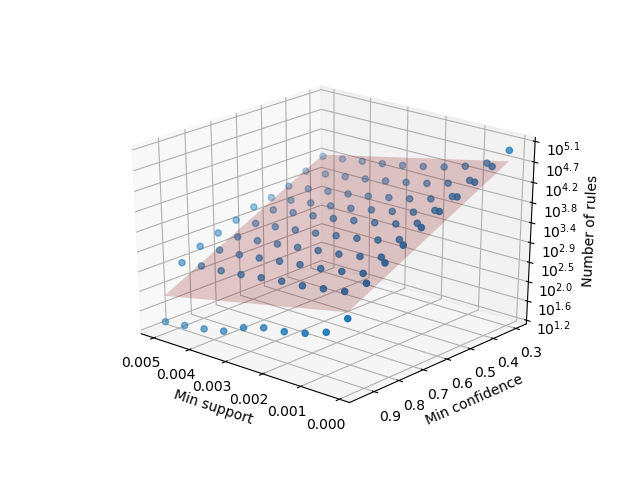
\includegraphics[width=0.95\textwidth]{images/results/spotify_num_rules.png}%
}

\subfloat[Number of rules with error bars]{%
  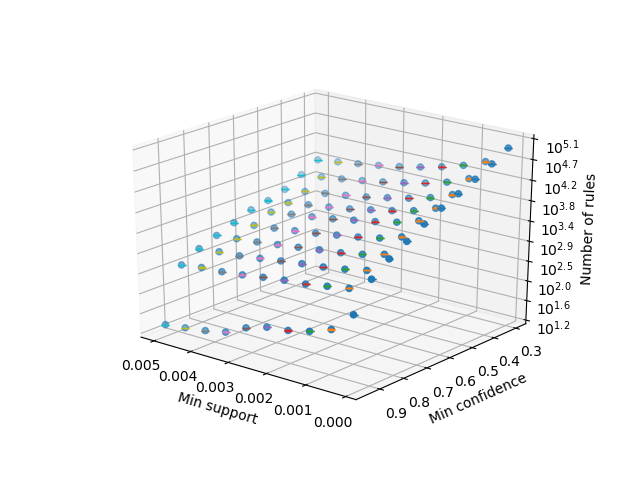
\includegraphics[width=0.95\textwidth]{images/results/spotify_num_rules_with_error_bars.png}%
}

\caption{Number of generated rules for Spotify measurements as a function of minimum support threshold and minimum confidence threshold}
\label{figure:number-of-rules-spotify}
\end{figure}


%\begin{figure}[htp]
%\subfloat[Facebook mobile application]{%
%  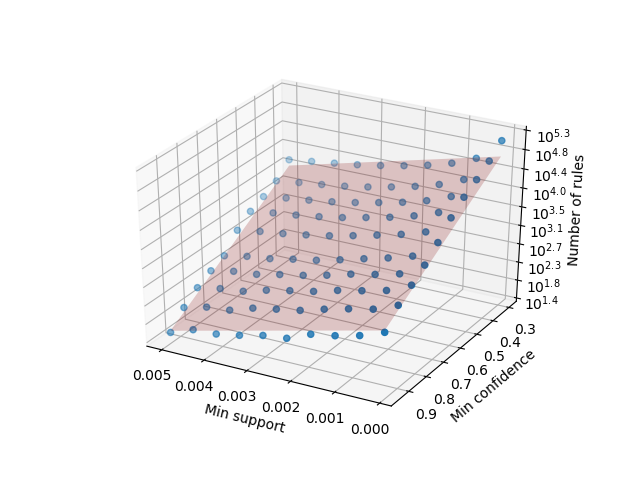
\includegraphics[width=\textwidth]{images/results/facebook_num_rules.png}%
%}
%\subfloat[Spotify mobile application]{%
%  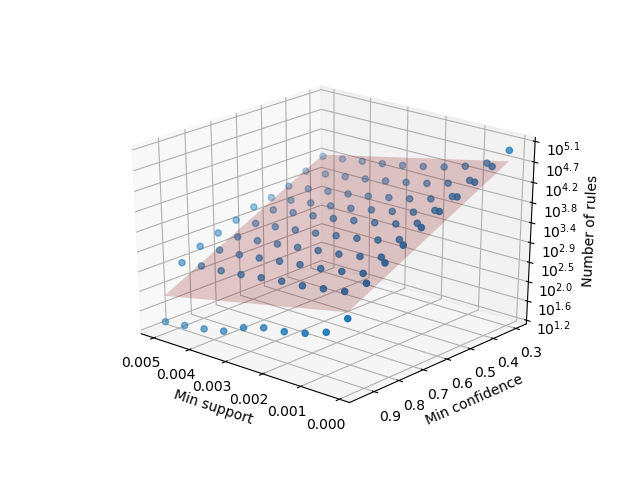
\includegraphics[width=\textwidth]{images/results/spotify_num_rules.png}%
%}
%\caption{Number of generated rules plotted as a function of minimum support threshold and minimum confidence threshold}
%\label{figure:number-of-ruless}
%\end{figure}

\begin{figure} %[htp]

\subfloat[Rule generation time with best fitting plane]{
  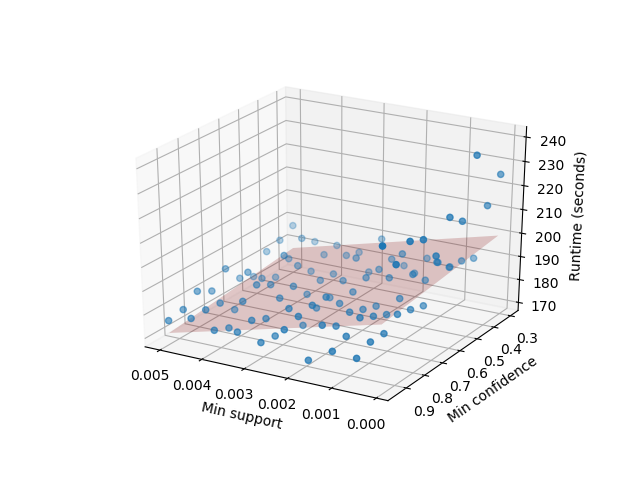
\includegraphics[width=0.95\textwidth]{images/results/facebook_runtimes.png}%
}

\subfloat[Rule generation time with error bars]{%
  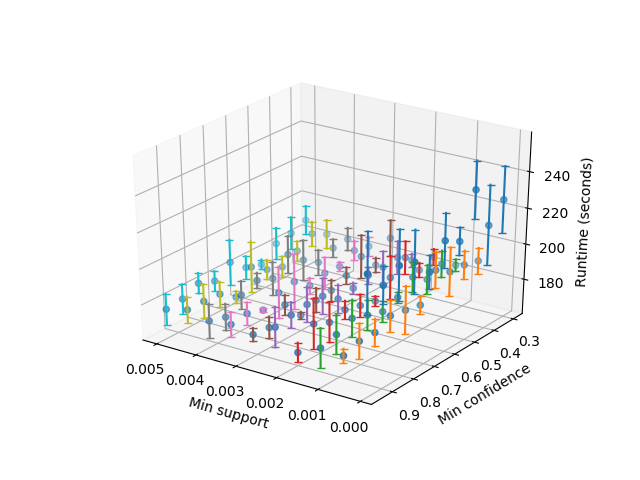
\includegraphics[width=0.95\textwidth]{images/results/facebook_runtimes_with_error_bars.png}%
}

\caption{Rule generation time for Facebook measurements as a function of minimum support threshold and minimum confidence threshold}
\label{figure:runtimes-facebook}
\end{figure}

In addition to the number of generated rules, another metric that is a good indicator for usability of the system, is the time taken to generate the association rules. To measure the time of the rule generation as a function of minimum support threshold and minimum confidence threshold, a similar set up as with the number of generated rules was used. Figure~\ref{figure:runtimes-facebook} shows these measurements for the Facebook application and Figure~\ref{figure:runtimes-spotify} shows the measurements for the Spotify application. Like before, the blue dots represent the average value in five measurements series of 100 measurement points. The red plane represents a plane that was fitted to the points using the least squares method. The size of the error in the error bars is again the standard deviation of the measurement at each measurement point.

The rule generation time increases as either axis approaches zero. The deviance is not huge however, as all the measured run times fall between 160 and 260 seconds. While this is a notable difference from the users perspective, the system remains usable even when the number of generated rules is in the order of $10^5$.   

\begin{figure} %[htp]

\subfloat[Rule generation time with best fitting plane]{
  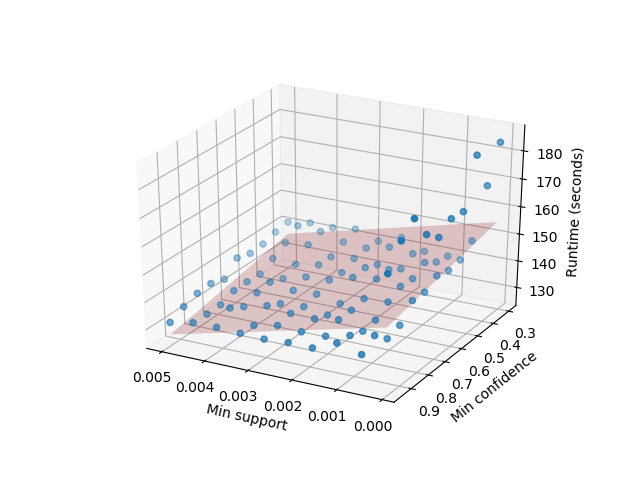
\includegraphics[width=0.95\textwidth]{images/results/spotify_runtimes.png}%
}

\subfloat[Rule generation time with error bars]{%
  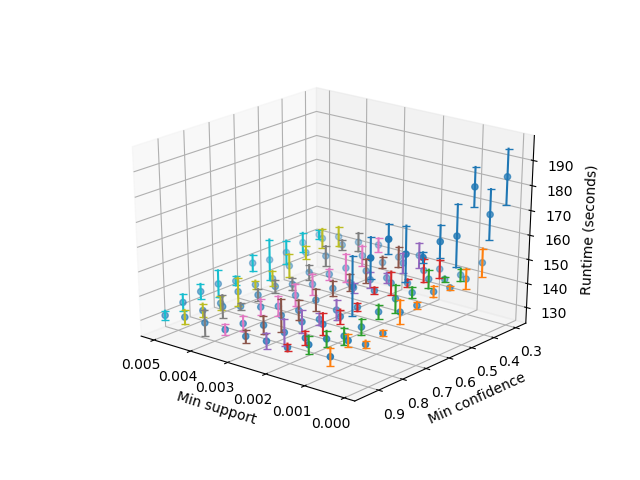
\includegraphics[width=0.95\textwidth]{images/results/spotify_runtimes_with_error_bars.png}%
}

\caption{Rule generation time for Spotify measurements as a function of minimum support threshold and minimum confidence threshold}
\label{figure:runtimes-spotify}
\end{figure}

All the experiments were conducted on a Spark cluster which had a single computing server. For each run, 45 CPU cores and 1500 gigabytes of memory were reserved. To mitigate the effect of any potential file server load, the dataset was stored in memory using Linux shared memory file system (/dev/shm). The dataset consisted of Carat samples from 22.6.2016 to 22.8.2016, the size of which was a little over 16 gigabytes.


%\begin{figure}[htp]
%\subfloat[Facebook mobile application]{%
%  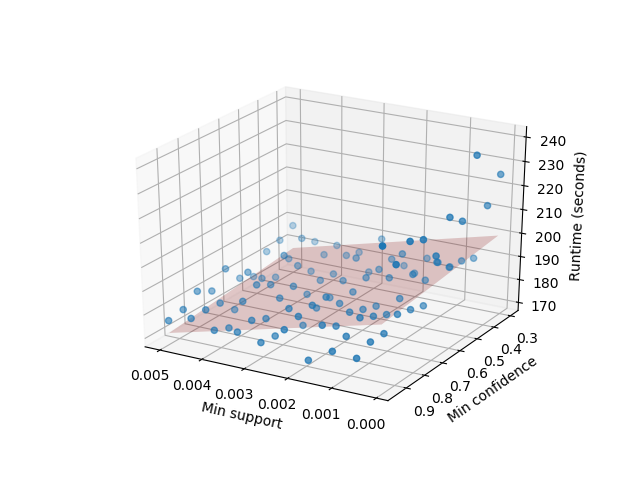
\includegraphics[width=\textwidth]{images/results/facebook_runtimes.png}%
%}
%\subfloat[Spotify mobile application]{%
%  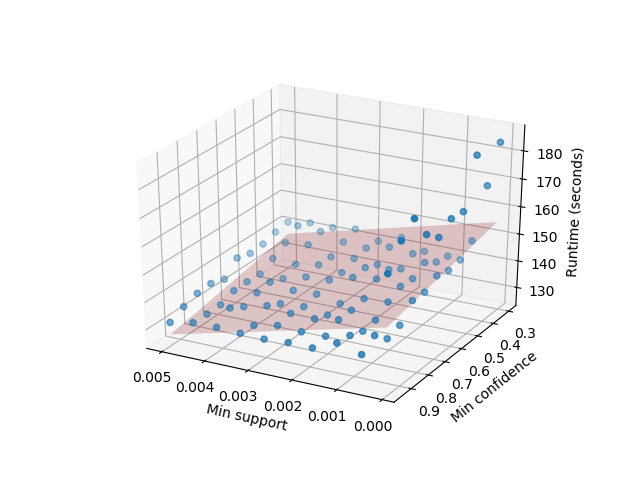
\includegraphics[width=\textwidth]{images/results/spotify_runtimes.png}%
%}
%\caption{Association rule generation time as a function of minimum support threshold and minimum confidence threshold}
%\label{figure:analysis-runtime}
%\end{figure}  

\subsection{Overview on Generated Rules}

For this section, four popular Android applications were selected to be inspected with the rule generation. The selected applications were 

\begin{itemize}
	\item com.facebook.katana
	\item com.google.android.chrome
	\item com.google.android.apps.photos
	\item com.spotify.music
\end{itemize}

%com.facebook.katana, com.google.android.chrome, com.google.android.apps.photos and com.spotify.music. 
To achieve comparable results, the minimum support threshold was fixed to 0.001 and the minimum confidence threshold was fixed to 0.5. Given that the least popular of these applications in the dataset used for this analysis contained little over 420 000 data points, a minimum support threshold of 0.001 means that for each generated rule, there should always be at least 420 data points supporting that rule. For each of these four applications, a total of six of the generated rules were selected for further inspection. These six rules were selected by taking the three most confident rules that predicted high energy consumption rate and the three most confident rules that predicted low energy consumption rate.  

Table~\ref{table:rules-facebook} shows the generated rules for the com.facebook.katana mobile application. Looking at the top three rules that predicted hight energy rate for the application, it seems that using HSDPA type mobile network connection and a high screen brightness were clearly connected to high energy consumption. When these two factors were combined with high battery temperature, we get the most confident of these three rules with a confidence score of 0.5811. As the highest confidence rule in this category had a confidence score of less than 0.6, one can say that there were no clear explanations of high energy consumption to be found by these variables for this particular application. Looking at the three most confident rules for low energy consumption, the common factors seem to be using WiFi connection, low battery temperature and low or medium low CPU usage. Notably, the rules for low energy consumption had significantly greater confidence than the rules for high energy consumption. The highest confidence for these three rules was 0.9985 while the lowest was 0.9964. 

\begin{table} \small%
\begin{tabular}{|p{5.0cm}|p{3.0cm}|p{2.0cm}|p{1.5cm}|p{0.3cm}| p{0.3cm}|}
\hline
Antecedents & Consequent & Confidence \\
\hline
	mobileNetType=hsdpa 		& & \\
	screen is 222 - 255			& rate is 0.011 - 1.0 & 0.5811 \\
	temperature is 35 - 88		& & \\
\hline
	mobileNetType=hsdpa			& & \\
	screen is 222 - 255			& & \\
	cpu is 0.39 - 0.62			& rate is 0.011 - 1.0 & 0.5464 \\
	voltage is 0 - 3			& & \\
	distance=no					& & \\
\hline
	mobileNetType=hsdpa			& & \\
	screen is 222 - 255			& rate is 0.011 - 1.0 & 0.5432 \\
	cpu is 0.39 - 0.62			& & \\
	voltage is 0 - 3			& & \\
\hline
	mobileNetType=unknown		& & \\
	screen is 222 - 255			& & \\
	wifiStrength is -99 - -69	& rate is 0.0 - 0.00017 & 0.9985 \\
	cpu is 0.0 - 0.39			& & \\
	temperature is 5 - 28		& & \\
	voltage is 3 - 4			& & \\
\hline
	mobileNetType=unknown		& & \\
	screen is 222 - 255			& & \\
	wifiStrength is -99 - -69	& rate is 0.0 - 0.00017 & 0.9974 \\
	wifiSpeed is 54 - 72		& & \\
	cpu is 0.39 - 0.62			& & \\
	temperature is 5 - 28		& & \\
	voltage is 0 - 3			& & \\
\hline
	mobileNetType=unknown		& & \\
	screen is 222 - 255			& & \\
	wifiSpeed is 0 - 54			& rate is 0.0 - 0.00017 & 0.9964 \\
	cpu is 0.39 - 0.62			& & \\
	temperature is 5 - 28		& & \\
	voltage is 3 - 4			& & \\
\hline
\end{tabular}
	\caption{Selected rules for the com.facebook.katana mobile application}
	\label{table:rules-facebook}
\end{table}

In Table~\ref{table:rules-android-photos} shows the selected rules for the com.google.android.apps.photos application. In this case, the factors that indicated high energy consumption were using GPRS for mobile networking, having weak WiFi singnal strength and low WiFi signal speed and low battery voltage. The low battery voltage may indicate a certain set of mobile devices that perform poorly when the other factors are also present. The confidence of these rules were reasonable, ranging from 0.7100 to 0.7074. The most confident rules for low energy consumption all had the common factors of using UTMS mobile network connection, high WiFi link speed, medium low CPU usage and weirdly enough, high screen brightness. 

\begin{table} \small%
\begin{tabular}{|p{5.0cm}|p{3.0cm}|p{2.0cm}|p{1.5cm}|p{0.3cm}| p{0.3cm}|}
\hline
Antecedents & Consequent & Confidence \\
\hline
	mobileNetType=gprs				& & \\
	wifiStrength is -100 - -68		& & \\
	wifiSpeed is 0 - 54				& & \\
	netType=wifi					& rate is 0.011 - 1.0 & 0.7100 \\
	voltage is 0 - 3				& & \\
	distance=no						& & \\
\hline
	mobileNetType=gprs				& & \\
	wifiStrength is -100 - -68		& & \\
	wifiSpeed is 0 - 54				&  rate is 0.011 - 1.0 & 0.7082 \\
	voltage is 0 - 3				& & \\
	distance=no						& & \\
\hline
	mobileNetType=gprs				& & \\
	wifiStrength is -100 - -68		& & \\
	wifiSpeed is 0 - 54				& rate is 0.011 - 1.0 & 0.7074 \\
	netType=wifi					& & \\
	voltage is 0 - 3				& & \\
\hline
	screen is 220 - 255				& & \\
	mobileNetType=utms				& & \\
	wifiSpeed is 144 - 6477		& rate is 0.0 - 0.0015 & 0.9966 \\
	wifiStrength is -68 - -59		& & \\
	cpu is 0.42 - 0.67				& & \\
\hline
	screen is 220 - 255				& & \\
	mobileNetType=utms				& & \\
	wifiSpeed is 144 - 6477		& rate is 0.0 - 0.0015 & 0.9965 \\
	wifiStrength is -68 - -59		& & \\
	cpu is 0.42 - 0.67				& & \\
	voltage is 3 - 4				& & \\
\hline
	screen is 220 - 255				& & \\
	mobileNetType=utms				& & \\
	wifiSpeed is 144 - 6477		& rate is 0.0 - 0.0015 & 0.9936 \\
	cpu is 0.42 - 0.67				& & \\
	voltage is 3 - 4				& & \\
\hline
\end{tabular}
	\caption{Selected rules for the com.google.android.apps.photos mobile application}
	\label{table:rules-android-photos}
\end{table}

Table~\ref{table:rules-chrome} shows the selected rules for the com.android.chrome mobile application. There were no rules, within the given confidence constraint, that predicted an energy consumption rate in the highest quantile, so instead the three top rules in the table are the three highest confidence rules that predicted an energy consumption rate in the third quantile within the samples where the Chrome application was running. Within the rules which predicted high energy consumption, common factors were high screen brightness, high battery temperature, fast WiFi link speed and using LTE type mobile networking. The confidence of these rules ranged from 0.6519 to 0.65. Looking at the rules which predicted low energy consumption, common factors were low battery temperature, fast WiFI link speed, mobile networking type UTMS and again, oddly enough, a high screen brightness. The confidence of the rules predicting low energy consumption were again very high, ranging from 0.9985 to 0.9964.   

\begin{table} \small%
\begin{tabular}{|p{5.0cm}|p{3.0cm}|p{2.0cm}|p{1.5cm}|p{0.3cm}| p{0.3cm}|}
\hline
Antecedents & Consequent & Confidence \\
\hline
	screen is 206 - 255 			& & \\
	wifiSpeed is 135 - 4728		& & \\ 
	temperature is 34 - 88  		& rate is 0.0046 - 0.011 &  0.6519 \\
	mobileNetType=lte				& & \\
	netType=wifi					& & \\
\hline
	screen is 206 - 255				& & \\
	wifiSpeed is 135 - 4728 		& rate is 0.0046 - 0.011 & 0.6506 \\
	temperature is 34 - 88			& & \\
	mobileNetType=lte				& & \\
\hline
	screen is 206 - 255				& & \\
	wifiSpeed is 135 - 4728 		& & \\
	temperature is 34 - 88			& rate is 0.0046 - 0.011  & 0.65 \\
	mobileNetType=lte				& & \\
	netType=wifi					& & \\
	distance=no						& & \\
\hline
	screen is 206 - 255				& & \\
	mobileNetType=utms				& & \\
	wifiSpeed is 135 - 4728		& rate is 0.0 - 0.0015 & 0.9893 \\
	wifiStrength is -68 - -59		& & \\
	voltage is 3 - 4				& & \\
\hline
	screen is 206 - 255				& & \\
	mobileNetType=utms				& & \\
	wifiSpeed is 135 - 4728		& rate is 0.0 - 0.0015 & 0.9822 \\
	temperature is 5 - 28			& & \\
	voltage is 3 - 4				& & \\
\hline
	screen is 206 - 255				& & \\
	mobileNetType=utms				& rate is 0.0 - 0.0015 & 0.9749 \\
	wifiSpeed is 135 - 4728		& & \\
	temperature is 5 - 28			& & \\
\hline
\end{tabular}
	\caption{Selected rules for the com.google.android.chrome mobile application}
	\label{table:rules-chrome}
\end{table}

In Table~\ref{table:rules-spotify} are listed the selected rules for the com.spotify.music mobile application. In the context of the rules that predict high energy consumption, factors high screen brightness, high WiFi link speed, quite low wiFi signal strength, medium high battery temperature and medium high CPU usage are all shared. Two out of three of these rules also share the factor mobile networking type LTE and low battery voltage. The confidence of these rules ranged from 0.8852 to 0.8821, which compared to the other application's high energy rules, seems very high. Among the rules that predicted low energy consumption, shared factors were mobile networking type UTMS, a medium high CPU usage, and a medium low wiFi signal strength. Factors that were shared by two out of the three rules included high screen brightness, low battery temperature and high WiFi link speed. The confidence score of all three of these rules was 1.0. 

\begin{table} \small%
\begin{tabular}{|p{5.0cm}|p{3.0cm}|p{2.0cm}|p{1.5cm}|p{0.3cm}| p{0.3cm}|}
\hline
Antecedents & Consequent & Confidence \\
\hline
	screen is 210 - 255 		& & \\
	wifiSpeed is 144 - 866		& & \\
	wifiStrength is -68 - -59	& & \\
	temperature is 34 - 60		& rate is 0.012 - 1.0 & 0.8852 \\
	cpu is 0.61 - 0.84			& & \\
	mobileNetType=lte			& & \\
	voltage is 0 - 3			& & \\
\hline
	screen is 210 - 255			& & \\
	wifiSpeed is 144 - 866		& & \\
	wifiStrength is -68 - -59	& rate is 0.012 - 1.0 & 0.8821 \\
	temperature is 34 - 60		& & \\
	cpu is 0.61 - 0.84			& & \\
	voltage is 0 - 3			& & \\
\hline
	screen is 210 - 255			& & \\
	wifiSpeed is 144 - 866		& & \\
	wifiStrength is -68 - -59	& rate is 0.012 - 1.0 & 0.8821 \\
	temperature is 34 - 60		& & \\
	cpu is 0.61 - 0.84			& & \\
	mobileNetType=lte			& & \\
\hline
	mobileNetType=utms			& & \\
	wifiSpeed is 144 - 866		& & \\
	wifiStrength is -68 - -59	& rate is 0.0 - 0.0016 & 1.0 \\
	cpu is 0.61 - 0.84			& & \\
	temperature is 12 - 28		& & \\
	voltage is 3 - 4			& & \\
\hline
	screen is 210 - 255			& & \\
	mobileNetType=utms			& & \\
	wifiStrength is -68 - -59	& rate is 0.0 - 0.0016 & 1.0 \\
	cpu is 0.61 - 0.84			& & \\
	temperature is 12 - 28		& & \\
\hline
	screen is 210 - 255			& & \\
	mobileNetType=utms			& & \\
	wifiSpeed is 144 - 866		& rate is 0.0 - 0.0016 & 1.0 \\
	wifiStrength is -68 - -59	& & \\
	cpu is 0.61 - 0.84			& & \\
\hline
\end{tabular}
	\caption{Selected rules for the com.spotify.music mobile application}
	\label{table:rules-spotify}
\end{table}

The generated example rules are generally not very intuitive and some of the relations, such as the contribution of high screen brightness to low energy consumption, are outright counter intuitive. On the bright side, the system is able to find rules with very high confidence even with a reasonably high support threshold of 0.001. The choice of application also seems to have a reasonable impact on the generated rules, which is promising for the usability of the system. Perhaps interesting is the fact that more confident rules seem to be generated for the low energy consumption than for the high energy consumption. Even if the system is not able to predict with any reasonable accuracy which factors lead to large levels of energy consumption when using a certain application, it might be useful to be able predict with acceptable accuracy which combinations of factors lead to low levels of energy consumption. At the very least, this kind of prediction could be a valuable addition to a recommendation system like the one described in~\cite{PELTONEN201671}.

\subsection{Discussion}

This thesis work has presented a method for generating association rules from Carat dataset in order to estimate how mobile device system settings and context factors impact the level of energy consumption of a mobile device when using a particular mobile application. These association rules reveal non-trivial and perhaps unexpected connections between these settings and context factor and the level of energy consumption within the context of multiple mobile applications. For some reason, the generated association rules that predict low levels of energy consumption, seem to have much higher confidence than the rules which predict high levels energy consumption. This may be due to various reasons. One reason might be, that while the association analysis seems to be able to capture at least some circumstances which consistently lead to low energy consumption, the system settings and context variables available within the Carat dataset are inadequate for explaining unusually high energy consumption levels. It could even be, that the users whose devices have high energy consumption are generally running multiple mobile applications at the same time, which would naturally generate more noise to data points coming from those users. One could potentially test this hypothesis by adding the number of running applications to the list of variables from which the association rules are generated from. If this was the case, then one would expect to see rules where high number of running applications predicts high energy consumption. 

Another goal of thesis work was to implement a web based interface, so that users could search these association rules easily. The implementation has two web servers that communicate to one another using a simple HTTP based API. The back end of the service resides on a Spark cluster where it can execute the analysis engine on user supplied parameters as requested. This way the data analysis can be wrapped inside a single exchange of HTTP request and response. The front end of the service handles all things related to the graphical user interface: rendering the search form, fetching the rules from the back end and rendering the results. The front end of the service can reside wherever as long as the service back end can be reached by HTTP. This two-tier architecture allows the remote use of computational resources of a Spark cluster without exposing the Spark cluster environment to potential security vulnerabilities that a globally accessible web server might impose.

The implementations of both the data analysis and the user interface could be further improved. First of all, due to performance reasons, the data set had to be limited to around 16 GB, which is more than an order of magnitude less than the whole amount of available data. It is quite possible that the association analysis might reveal more fine grained dependencies between the context factors and system settings and the energy consumption of a device, if the analysis was performed using more of the available data. Different discretization strategies for the data might also affect the generated rules. Discretization of most numerical variables was done using quite an arbitrary number of percentiles, namely four. The implementation could easily be extended to allow the user to specify the number percentiles used in the discretization.

The user interface could be improved in multiple ways. The user interface does not show the units of measurement nor does it show values of the break points of the percentiles, which could give the user a clearer sense of how a certain value range of a variable compares to the average value of the variable. Rendering of the rules could also be improved. Paging of the rules should definitely be implemented because browsing through as many as thousands of rules in a single page is cumbersome. The user could also benefit from a searching and filtering functionality in the front end of the service to be able quickly find the rules that the user considers interesting.
     

\section{Conclusion}

%This thesis work has presented a method for generating association rules from Carat dataset in order to estimate how mobile device system settings and context factors impact the level of energy consumption of a mobile device when using a particular mobile application. These association rules reveal non-trivial and perhaps unexpected connections between these settings and context factor and the level of energy consumption within the context of multiple mobile applications. For some reason, the generated association rules that predict low levels of energy consumption, seem to have much higher confidence than the rules which predict high levels energy consumption. This may be due to various reasons. One reason might be, that while the association analysis seems to be able to capture at least some circumstances which consistently lead to low energy consumption, the system settings and context variables available within the Carat dataset are inadequate for explaining unusually high energy consumption levels. It could even be, that the users whose devices have high energy consumption are generally running multiple mobile applications at the same time, which would naturally generate more noise to data points coming from those users. One could potentially test this hypothesis by adding the number of running applications to the list of variables from which the association rules are generated from. If this was the case, then one would expect to see rules where high number of running applications predicts high energy consumption. 

%Another goal of thesis work was to implement a web based interface, so that users could search these association rules easily. The implementation has two web servers that communicate to one another using a simple HTTP based API. The back end of the service resides on a Spark cluster where it can execute the analysis engine on user supplied parameters as requested. This way the data analysis can be wrapped inside a single exchange of HTTP request and response. The front end of the service handles all things related to the graphical user interface: rendering the search form, fetching the rules from the back end and rendering the results. The front end of the service can reside wherever as long as the service back end can be reached by HTTP. This two-tier architecture allows the remote use of computational resources of a Spark cluster without exposing the Spark cluster environment to potential security vulnerabilities that a globally accessible web server might impose.

%The implementations of both the data analysis and the user interface could be further improved. First of all, due to performance reasons, the data set had to be limited to around 16 GB, which is more than an order of magnitude less than the whole amount of available data. It is quite possible that the association analysis might reveal more fine grained dependencies between the context factors and system settings and the energy consumption of a device, if the analysis was performed using more of the available data. Different discretization strategies for the data might also affect the generated rules. Discretization of most numerical variables was done using quite an arbitrary number of percentiles, namely four. The implementation could easily be extended to allow the user to specify the number percentiles used in the discretization. 

%The user interface could be improved in multiple ways. The user interface does not show the units of measurement nor does it show values of the break points of the percentiles, which could give the user a clearer sense of how a certain value range of a variable compares to the average value of the variable. Rendering of the rules could also be improved. Paging of the rules should definitely be implemented because browsing through as many as thousands of rules in a single page is cumbersome. The user could also benefit from a searching and filtering functionality in the front end of the service to be able quickly find the rules that the user considers interesting. 

%This thesis work shows that the association analysis can effectively be applied to the domain of mobile device energy consumption modelling. This work also summarises the theoretical background of the state of the art methods used in association analysis and how to apply these methods using the MapReduce programming model. The performance evaluation aspect of the association rule generation process is also discussed and results of the evaluation are presented. Additional work is still needed to optimize the performance of the analysis engine and the usability of the user interface and to find out how different data discretization approaches affect the generated association rules. 

This thesis work has shows that the association analysis can effectively be applied to the domain of mobile device energy consumption modelling. Additionally, an implementation of a web based prototype for a developer API for the Carat dataset has been presented. The current state of the research of mobile device energy modelling as well as the relevant parts of the theory of association analysis have been reviewed.

The Carat data consists of samples which are collected from users of the Carat mobile application for the purpose collaborative energy modelling of mobile devices. Each sample contains a list of currently running mobile applications, energy consumption rate, CPU usage, travel distance, battery temperature, battery voltage, screen brightness, used mobile network technology, type of network,  WiFi signal strength, and WiFi connection speed of the mobile device. This thesis has described in detail each of these variables as well as the discretization and preprocessing of the data that must be performed in order to make the association rule discovery applicable. In summary, the variables have been divided to either three or four bins of equal mass. Some assumptions about the feasible range of the variables have been applied in preprocessing stage to exclude potentially corrupted data points.

This work has presented the essential theoretical background of the association analysis. It has introduced the FP-growth algorithm and the associated data structure FP-tree as a way of discovering frequent patterns from a dataset. It has also discussed how association rules can be generated from the frequent patterns without having to consider all candidate rules, giving an outline of an algorithm for pruning candidate rule search tree.

This thesis has shown how to implement a web based query engine that can be used to discover association rules based on the Carat data. The implementation has three major components, an analysis engine which handles all data analysis tasks, a back-end web server that uses the analysis engine as a service and exposes a JSON based HTTP API, and a service front-end that handles all user input and uses the API of the back-end server as a service for generating the association rules. The analysis engine has been built using Spark programming framework and specifically MLlib, a machine learning library for Spark which implements a parallel and distributed FP-growth algorithm.

The resulting association rules generated from the Carat data are somewhat promising. The analysis engine is consistently able to find high confidence rules from various different mobile applications. It seems however, that rules predicting high energy consumption are overall more rare and less confident than the rules which predict low or near average energy consumption. This thesis suggests some potential reasons as to why this may be the case. In order to evaluate the performance of the implementation, the runtime and the number generated rules have been measured as a function of the minimum confidence and minimum support thresholds of the association analysis for two popular Android mobile applications. The evaluation shows that the runtime of the analysis clearly depends on these variables, which is to be expected. While the runtime of the analysis shows a clear decreasing trend along both the minimum confidence threshold and the minimum support threshold axes, the magnitude of the analysis runtime does not change even when small values for these variables are used. A more problematic result from the usage point of view is the number of generated rules. Similarly to the runtime, it shows a clear decreasing trend along both the minimum support threshold and the minimum confidence threshold axes. Unlike the the runtime however, the number of generated rules ranges from as low as a dozen to tens of thousands. 

Further work is needed in order to improve the implementation of the search engine. The current implementation cannot handle tens of thousands of generated rules in a user friendly way. Additional methods should be considered for finding the interesting or important rules. It is also unintuitive that the user must specify the minimum support threshold and the minimum confidence threshold for the algorithm or settle with arbitrary default values. The engine should ideally be able to guess or iteratively find reasonable values for these variables based on the user preferences. Additionally, the effect of increasing or decreasing the number of discretization percentiles on the generated rules should be studied, or alternatively the user could be allowed to specify the number of percentiles for each of the variables. Further optimizing the implementation or performing experiments with more computing capacity could potentially reveal more intricate association rules.                

             


% --- References ---
%
% bibtex is used to generate the bibliography. The babplain style
% will generate numeric references (e.g. [1]) appropriate for theoretical
% computer science. If you need alphanumeric references (e.g [Tur90]), use
%
% \bibliographystyle{babalpha-lf}
%
% instead.

\bibliographystyle{babplain-lf}
\bibliography{references-en}


% --- Appendices ---

% uncomment the following

% \newpage
% \appendix
% 
% \section{Example appendix}

\end{document}